C) The general case.

Let \(V \in \mathcal{F}(E)\) . Denote by \(p_V\) the canonical mapping of E onto E/V, and by \(Q_V\) the positive quadratic form \(Q \circ {}^t p_V\) on \((E/V)'\) ; finally, let \(\mu_V\) be the measure on E/V with Fourier transform \(e^{-Q_V/2}\) (cf.~B)). If \(W \in \mathcal{F}(E)\) is contained in V, then \(p_V = p_{\text{VW}} \circ p_W\) , whence \(Q_V = Q_W \circ {}^t p_{\text{VW}}\) ; by formula (4) of No.~3, the measure \(p_{\text{VW}}(\mu_W)\) has as Fourier transform the function \((e^{-Q_W/2}) \circ {}^t p_{\text{VW}} = e^{-Q_V/2}\) , hence is equal to \(\mu_V\) . The family \((\mu_V)_{V \in \mathcal{F}(E)}\) is therefore a promeasure \(\mu\) on E. Formula (5) of No.~3 shows that \(\mathcal{F}\mu\) is equal to \(e^{-Q/2}\) .

DEFINITION 2. --- Let E be a locally convex space. For every positive quadratic form Q on \(E'\) , the promeasure on E whose Fourier transform is equal to \(e^{-Q/2}\) is called the Gaussian promeasure on E with variance Q, and is denoted \(\Gamma_{Q}\) . A promeasure \(\mu\) on E is said to be Gaussian if there exists a positive quadratic form Q on \(E'\) such that \(\mu = \Gamma_{Q}\) .

By an abuse of language, a bounded measure \(\mu\) on E will be said to be Gaussian with variance Q if the associated promeasure \(\widetilde{\mu}\) is equal to \(\Gamma_{Q}\) .

Remarks. --- 1) Let E be a finite-dimensional vector space, and let \(\mu\) be a positive measure on E of mass 1, such that every linear form on E belongs to \(\mathcal{L}^{2}(\mathrm{E},\mu)\) . One defines an element \(m\) of E and a positive quadratic form V on \(\mathrm{E}'\) by the formulas

\[
\langle m, x ^ {\prime} \rangle = \int_ {\mathbb {E}} \langle x, x ^ {\prime} \rangle d \mu (x), \quad \mathrm{V} (x ^ {\prime}) = \int_ {\mathbb {E}} \langle x - m, x ^ {\prime} \rangle^ {2} d \mu (x).
\]

In the traditional terminology of Probability Theory, m is called the mean and V the variance of \(\mu\) ; \(\mu\) is said to be centered if m = 0.

Now let \(a\) be an element of \(\mathbf{E}\) and \(\mathbf{Q}\) a positive quadratic form on \(\mathbf{E}'\) . Let us denote by \(\Gamma_{a,\mathbf{Q}}\) the image of the measure \(\Gamma_{\mathbf{Q}}\) under the translation \(x \mapsto x + a\) . It is easily seen that \(\Gamma_{a,\mathbf{Q}}\) is a positive measure on \(\mathbf{E}\) of mass 1, with Fourier transform \(x' \mapsto e^{i\langle a,x'\rangle - \frac{1}{2}\mathbf{Q}(x')}\) and mean \(a\) . Moreover, Prop. 6 below implies that \(\mathbf{Q}\) is the variance of \(\Gamma_{a,\mathbf{Q}}\) . One traditionally says that \(\Gamma_{a,\mathbf{Q}}\) is the Gaussian measure with mean \(a\) and variance \(\mathbf{Q}\) , and that \(\Gamma_{\mathbf{Q}} = \Gamma_{0,\mathbf{Q}}\) is the centered Gaussian measure with variance \(\mathbf{Q}\) . Since we shall only be considering centered Gaussian measures, we shall omit this qualifier.

\begin{enumerate}
\def\labelenumi{\arabic{enumi})}
\setcounter{enumi}{1}
\item
  Let \(\mathbf{Q}\) be a quadratic form on the dual \(\mathbf{E}'\) of a locally convex space \(\mathbf{E}\) . If there exists a promeasure on \(\mathbf{E}\) with Fourier transform \(e^{-\mathbf{Q} / 2}\) , the quadratic form \(\mathbf{Q}\) is necessarily positive: for, the function \(e^{-\mathbf{Q} / 2}\) is bounded on \(\mathbf{E}'\) ; therefore, for every \(x' \in \mathbf{E}'\) , the function \(t \mapsto e^{-t^2\mathbf{Q}(x') / 2} = e^{-\mathbf{Q}(tx') / 2}\) on \(\mathbf{R}\) is bounded, whence \(\mathbf{Q}(x') \geqslant 0\) .
\item
  The dual of \(\mathbf{R}\) is canonically isomorphic to \(\mathbf{R}\) and the positive quadratic forms on \(\mathbf{R}\) are the functions of the form \(t \mapsto at^2\) with \(a \geqslant 0\) . Therefore, there exists for every \(a \geqslant 0\) one and only bounded measure \(\gamma_a\) on \(\mathbf{R}\) whose Fourier transform is equal to the function \(t \mapsto e^{-at^2/2}\) ; by an abuse of language, \(\gamma_a\) is said to be the Gaussian measure on \(\mathbf{R}\) with variance \(a\) .
\end{enumerate}

The Fourier transform of \(\gamma_0\) is the constant 1, whence \(\gamma_0 = \varepsilon_0\) (unit mass at the origin of \(\mathbf{R}\) ). Suppose \(a > 0\) and denote by \(u_a\) the linear mapping \(x \mapsto a^{1/2}x\) ; then \(\mathcal{F}\gamma_a = \mathcal{F}\gamma_1 \circ {}^t u_a\) , whence \(\gamma_a = u_a(\gamma_1)\) . Lemma 2 shows that \(\gamma_1\) is the measure with density \(x \mapsto (2\pi)^{-1/2} e^{-x^2/2}\) with respect to Lebesgue measure; from this, one easily deduces

\[
d \gamma_ {a} (x) = (2 \pi a) ^ {- 1 / 2} e ^ {- x ^ {2} / 2 a} d x.\tag{15}
\]

The image of a Gaussian promeasure under a continuous linear mapping is a Gaussian promeasure. More precisely, we have the following result:

PROPOSITION 5. --- Let E and \(E_{1}\) be two locally convex spaces, and u a continuous linear mapping of E into \(E_{1}\) . Let Q be a positive quadratic form on \(E'\) , and \(Q_{1}\) the positive quadratic form \(Q \circ {}^{t}u\) on \(E_{1}'\) . Then \(u(\Gamma_{Q}) = \Gamma_{Q_{1}}\) .

Set \(\mu = u(\Gamma_{\mathbb{Q}})\) . By formula (4) of No.~3,

\[
\mathcal {F} \mu = \left(\mathcal {F} \Gamma_ {\mathrm{Q}}\right) \circ {} ^ {t} u = e ^ {- \mathrm{Q} / 2} \circ {} ^ {t} u = e ^ {- \mathrm{Q} _ {1} / 2} = \mathcal {F} \Gamma_ {\mathrm{Q} _ {1}},
\]

whence \(\mu = \Gamma_{\mathbf{Q}_1}\) by Prop. 3 of No.~3.

COROLLARY. --- Let E be a locally convex space and Q a positive quadratic form on \(E'\) . For every \(x' \in E'\) , the image of \(\Gamma_{Q}\) under \(x'\) is the Gaussian measure on R with variance \(\mathrm{Q}(x')\) .

PROPOSITION 6. --- Let E be a locally convex space, and \(\mu\) a Gaussian measure on E, with variance Q. For every integer \(n \geqslant 0\) and every \(x' \in \mathbf{E}'\) , one has the relations

\[
\int_ {\mathrm{E}} | \langle x, x ^ {\prime} \rangle | ^ {n} d \mu (x) = \pi^ {- 1 / 2} 2 ^ {n / 2} \Gamma \Big (\frac {n + 1}{2} \Big) \mathrm{Q} (x ^ {\prime}) ^ {n / 2}\tag{16}
\]

\[
\int_ {\mathrm{E}} \langle x, x ^ {\prime} \rangle^ {2 n} d \mu (x) = \frac {(2 n) !}{2 ^ {n} n !} \mathrm{Q} (x ^ {\prime}) ^ {n}\tag{17}
\]

\[
\int_ {\mathrm{E}} \langle x, x ^ {\prime} \rangle^ {2 n + 1} d \mu (x) = 0.\tag{18}
\]

In particular,

\[
\int_ {\mathrm{E}} \langle x, x ^ {\prime} \rangle^ {2} d \mu (x) = \mathrm{Q} (x ^ {\prime}) \qquad (x ^ {\prime} \in \mathrm{E} ^ {\prime}).\tag{19}
\]

If these formulas are true for an element \(x'\) of \(E'\) , then they are true for all of its multiples \(t \cdot x'\) (with t real). We may therefore content ourselves with establishing them when \(\mathrm{Q}(x')\) is equal to 0 or 1.

\begin{enumerate}
\def\labelenumi{\alph{enumi})}
\item
  Suppose \(\mathrm{Q}(x') = 0\) . The measure \(x'(\mu)\) is equal to \(\gamma_{0} = \varepsilon_{0}\) , therefore \(x'\) is zero \(\mu\) -almost everywhere; the formulas (16) to (19) are then obvious.
\item
  Suppose \(\mathrm{Q}(x') = 1\) , whence \(x'(\mu) = \gamma_{1}\) . Then
\end{enumerate}

\[
\int_ {\mathbf {E}} | \langle x, x ^ {\prime} \rangle | ^ {n} d \mu (x) = \int_ {\mathbf {R}} | t | ^ {n} d \gamma_ {1} (t) = (2 \pi) ^ {- 1 / 2} \int_ {\mathbf {R}} | t | ^ {n} e ^ {- t ^ {2} / 2} d t
\]

and (16) follows immediately from (6) (No 4, Lemma 1). Similarly, formulas (17) and (18) follow from (7) and (8). Finally, (19) is obtained by setting \(n = 1\) in (17).

We can now prove a converse of the Cor. of Prop. 5.

PROPOSITION 7. --- Let E be a locally convex space and \(\mu\) a promeasure on E. Suppose that \(x'(\mu)\) is a Gaussian measure on R for every \(x' \in E'\) . Then \(\mu\) is a Gaussian promeasure on E.

For every \(x' \in \mathrm{E}'\) , let \(\mathbf{Q}(x')\) be the variance of the Gaussian measure \(x'(\mu)\) on \(\mathbf{R}\) . One has \(x'(\mu) = \gamma_{\mathbf{Q}(x')}\) , whence

\[
(\mathcal {F} \mu) (x ^ {\prime}) = \int_ {\mathbf {R}} e ^ {i t \cdot 1} d \gamma_ {Q (x ^ {\prime})} (t) = e ^ {- Q (x ^ {\prime}) \cdot 1 ^ {2} / 2}
\]

by the definition of \(\mathcal{F}\mu\) (No.~3, formula (2)). In other words, \(\mathcal{F}\mu = e^{-Q/2}\) , and it remains to prove that \(Q\) is a positive quadratic form on \(E'\) .

For every closed linear subspace V of E with finite codimension, denote by \(p_{V}\) the canonical mapping of E onto E/V, by \(\mu_{V}\) the measure \(p_{\mathrm{V}}(\mu)\) on E/V, and set \(Q_{V} = Q \circ {}^{t} p_{V}\) . Since \(E' = \bigcup_{V \in \mathcal{F}(E)} \operatorname{Im}({}^{t} p_{V})\) and \({}^{t} p_{V}\) is injective, it suffices to prove that \(Q_{V}\) is a positive quadratic form on \((\mathrm{E}/\mathrm{V})'\) .

Let \(u \in (\mathrm{E}/\mathrm{V})'\) and \(x' = {}^{t} p_{\mathrm{V}}(u)\) . We have

\[
u (\mu_ {\mathrm{V}}) = u \big (p _ {\mathrm{V}} (\mu) \big) = x ^ {\prime} (\mu) = \gamma_ {\mathrm{Q} (x ^ {\prime})};
\]

Prop. 6 then implies

\[
\mathrm{Q} _ {\mathrm{V}} (u) = \mathrm{Q} (x ^ {\prime}) = \int_ {\mathbf {R}} t ^ {2} d \gamma_ {\mathrm{Q} (x ^ {\prime})} (t) = \int_ {\mathrm{E} / \mathrm{V}} u (x) ^ {2} d \mu_ {\mathrm{V}} (x),
\]

thus \(Q_V\) is a positive quadratic form on \((E/V)'\) .

\subsection{Examples of Gaussian promeasures}

\begin{enumerate}
\def\labelenumi{\arabic{enumi})}
\tightlist
\item
  Let E be a real Hilbert space. The mapping \(x' \mapsto \|x'\|^2\) is a positive quadratic form on \(E'\) . The corresponding Gaussian promeasure is called the canonical Gaussian promeasure on E. It can be shown that this promeasure is not a measure if E is infinite-dimensional.
\end{enumerate}

Let \(A\) be a continuous linear operator on \(\mathbf{E}\) . The mapping \(x' \mapsto \|{}^{t} A \cdot x'\|^2\) is a positive quadratic form on \(\mathbf{E}'\) . The corresponding promeasure \(\mu_A\) on \(\mathbf{E}\) is a measure if and only if \(A\) is a Hilbert--Schmidt operator (cf.~No.~11, Cor. 2 of Th. 3).

\begin{enumerate}
\def\labelenumi{\arabic{enumi})}
\setcounter{enumi}{1}
\tightlist
\item
  Kernels of positive type. Let T be a set and \(E = R^{T}\) the vector space of real functions on T, equipped with the topology of pointwise convergence. For every \(t \in T\) , one denotes by \(\varepsilon_{t}\) the linear form \(f \mapsto f(t)\) on E. The family \((\varepsilon_{t})_{t \in \mathbb{T}}\) is a basis of \(E'\) (TVS, II, §6, No.~6, Cor. 2 of Prop. 8).
\end{enumerate}

One calls (real) kernel of positive type on T every real-valued function K on \(T \times T\) satisfying the relations

\[
\mathbf {K} (t, t ^ {\prime}) = \mathbf {K} (t ^ {\prime}, t) \quad \text { for } t, t ^ {\prime} \text { in } \mathbf {T},\tag{20}
\]

\[
\sum_ {i, j = 1} ^ {p} c _ {i} c _ {j} \mathrm{K} (t _ {i}, t _ {j}) \geqslant 0\tag{21}
\]

for any positive integer \(p\) , elements \(t_1, \ldots, t_p\) of \(T\) , and real numbers \(c_1, \ldots, c_p\) . If this is so, the formula

\[
q \left(\sum_ {t \in \mathrm{T}} c _ {t} \varepsilon_ {t}\right) = \sum_ {t, t ^ {\prime} \in \mathrm{T}} c _ {t} c _ {t ^ {\prime}} \mathrm{K} (t, t ^ {\prime})\tag{22}
\]

defines a positive quadratic form on \(\mathbf{E}'\) . Conversely, if \(q\) is a positive quadratic form on \(\mathbf{E}'\) , then the formula

\[
\mathbf {K} (t, t ^ {\prime}) = \frac {1}{2} [ q (\varepsilon_ {t} + \varepsilon_ {t ^ {\prime}}) - q (\varepsilon_ {t}) - q (\varepsilon_ {t ^ {\prime}}) ]\tag{23}
\]

defines a kernel K of positive type on T. One thus obtains two mutually inverse bijections between the set of kernels of positive type on T, and that of the positive quadratic forms on \(E'\) .

Let K be a kernel of positive type on T, and q the associated quadratic form on \(E'\) . The Gaussian promeasure on E with variance q is also called the Gaussian promeasure on E with covariance K. If T is countable, Prop. 2 of No.~1 implies that this promeasure is a measure.

\begin{enumerate}
\def\labelenumi{\arabic{enumi})}
\setcounter{enumi}{2}
\tightlist
\item
  Let \(\mathbf{T}\) be a countable set. A kernel \(\delta\) on \(\mathbf{T}\) of positive type is defined by setting
\end{enumerate}

\[
\delta (t, t ^ {\prime}) = \left\{ \begin{array}{l l} 1 & \text { if } t = t ^ {\prime} \\ 0 & \text { if } t \neq t ^ {\prime}. \end{array} \right.\tag{24}
\]

The corresponding quadratic form is given by \(q\left(\sum_{t \in \mathbb{T}} c_t \varepsilon_t\right) = \sum_{t \in \mathbb{T}} c_t^2\) . For every \(t \in \mathbb{T}\) , let us denote by \(\mu_t\) the Gaussian measure on \(\mathbf{R}\) with variance 1;

one shows easily that the Gaussian measure on \(\mathbf{R}^{\mathrm{T}}\) with covariance \(\delta\) is equal to \(\bigotimes_{t\in T}\mu_t\) .

\begin{enumerate}
\def\labelenumi{\arabic{enumi})}
\setcounter{enumi}{3}
\tightlist
\item
  Let \(n \geqslant 1\) be an integer. A square matrix \(C = (c_{ij})\) of order \(n\) is said to be positive symmetric if it is symmetric and \(\sum_{i,j=1}^{n} c_{ij} x_i x_j \geqslant 0\) for any real \(x_1, \ldots, x_n\) ; it comes to the same to say that the mapping \((i,j) \mapsto c_{ij}\) is a kernel of positive type on the set \(\{1,2,\ldots,n\}\) . We may therefore speak of the Gaussian measure \(\gamma_C\) on \(\mathbf{R}^n\) , with covariance \(C\) ; it is characterized by the formula
\end{enumerate}

\[
\int_ {\mathbf {R} ^ {n}} e ^ {i (x _ {1} t _ {1} + \dots + x _ {n} t _ {n})} d \gamma_ {C} (t _ {1}, \dots , t _ {n}) = \exp \left(- \frac {1}{2} \sum_ {j, k = 1} ^ {n} c _ {j k} x _ {j} x _ {k}\right),\tag{25}
\]

for \(x_{1}, \ldots, x_{n}\) real. From Prop. 6 of No.~5 (formula (19)), one deduces

\[
\int_ {\mathbf {R} ^ {n}} t _ {j} t _ {k} d \gamma_ {C} (t _ {1}, \dots , t _ {n}) = c _ {j k} \quad (1 \leqslant j, k \leqslant n).\tag{26}
\]

From Prop. 5 of No.~5, one deduces the formula

\[
u (\gamma_ {C}) = \gamma_{U C\,{}^{t}U}  ,\tag{27}
\]

where u is a linear mapping of \(R^{n}\) into \(R^{m}\) with matrix U. Moreover, one sees easily (cf.~the first part of the proof of Prop. 4 of No.~5) that if \(I_{n}\) is the identity matrix of order n, then the measure \(\gamma_{I_{n}}\) admits the density

\[
(2 \pi) ^ {- n / 2} \exp \left(- \frac {1}{2} (t _ {1} ^ {2} + \dots + t _ {n} ^ {2})\right)
\]

with respect to the Lebesgue measure \(\lambda_{n}\) on \(\mathbf{R}^{n}\) .

We are going to show that if the matrix \(C\) is invertible, with inverse \(D = (d_{jk})\) , then

\[
\begin{array}{l} d \gamma_ {C} (t _ {1}, \dots , t _ {n}) = \\ (2 \pi) ^ {- n / 2} (\det D) ^ {1 / 2} \left(\exp \left(- \frac {1}{2} \sum_ {j, k = 1} ^ {n} d _ {j k} t _ {j} t _ {k}\right)\right) d t _ {1} \dots d t _ {n}. \end{array}\tag{28}
\]

For, if \(C\) is invertible, the quadratic form \(q\) on \(\mathbf{R}^n\) defined by

\[
q (x _ {1}, \dots , x _ {n}) = \sum_ {j, k = 1} ^ {n} c _ {j k} x _ {j} x _ {k}
\]

is nondegenerate. Using the existence of a basis of \(R^{n}\) orthonormal for q, one proves the existence of a square matrix U of order n such that \(C = U \cdot {}^{t}U\) , whence \(\gamma_{C} = u(\gamma_{I_{n}})\) by (27) (where u denotes the automorphism of \(R^{n}\) with matrix U). Let Q be the quadratic form on \(R^{n}\) defined by

\[
Q (t _ {1}, \dots , t _ {n}) = t _ {1} ^ {2} + \dots + t _ {n} ^ {2};
\]

then

\[
\gamma_ {I _ {n}} = (2 \pi) ^ {- n / 2} e ^ {- Q / 2} \cdot \lambda_ {n},
\]

whence

\[
u (\gamma_ {I _ {n}}) = (2 \pi) ^ {- n / 2} e ^ {- (\mathrm{Q} \circ u ^ {- 1}) / 2} \cdot u (\lambda_ {n}).\tag{29}
\]

It is immediate that the quadratic form \(\mathbf{Q} \circ u^{-1}\) on \(\mathbf{R}^n\) takes the value \(\sum_{j,k=1}^{n} d_{jk} t_j t_k\) at the point \((t_1, \ldots, t_n)\) , and Prop. 15 of Ch. VII, §1, No.~10 shows that

\[
u (\lambda_ {n}) = (\det U) ^ {- 1} \cdot \lambda_ {n} = (\det D) ^ {1 / 2} \cdot \lambda_ {n}.\tag{30}
\]

Formula (28) then follows from this.

\subsection{Wiener measure}

In this No., we denote by T the interval \([0,1]\) of R and by H the Hilbert space of real functions on T square-integrable with respect to Lebesgue measure, where the scalar product is denoted \((f|g)\) . We also denote by C the space of continuous real functions on T tending to 0 at the point 0; we equip C with the norm \(\|f\| = \sup_{t \in T} |f(t)|\) . The compact interval \([0,1] = T \cup \{0\}\) is the Alexandroff compactification of the locally compact but noncompact interval T; consequently, the set of continuous functions on T with compact support is dense in C, and the dual of C may be identified with the space \(M^{1}\) of bounded measures (not necessarily positive) on T (Ch. III, §1, No.~8, Def. 3).

For every function \(f \in \mathcal{H}\) , one defines a function \(Pf\) on \(T\) by

\[
(P f) (t) = \int_ {0} ^ {t} f (x) d x = (f | \mathrm{I} _ {t}),\tag{31}
\]

where \(I_{t}\) is the characteristic function of the interval \([0, t]\) . The Cauchy--Schwarz inequality implies the inequalities

\[
| (P f) (t) | \leqslant \| f \| _ {2} \cdot t ^ {1 / 2}\tag{32}
\]

\[
\left| (P f) (t) - (P f) \left(t ^ {\prime}\right) \right| \leqslant \| f \| _ {2} \cdot \left| t - t ^ {\prime} \right| ^ {1 / 2}\tag{33}
\]

consequently, \(Pf\) belongs to \(\mathcal{C}\) , and the linear mapping \(P\) of \(\mathcal{H}\) into \(\mathcal{C}\) is continuous with norm \(\leqslant 1\) .

Let us identify the Hilbert space \(\mathcal{H}\) with its dual (TVS, V, §1, No.~7, Th. 3), and denote by \(\Pi : \mathcal{M}^1 \to \mathcal{H}\) the transpose of \(P: \mathcal{H} \to \mathcal{C}\) . For every measure \(\mu \in \mathcal{M}^1\) and every function \(f \in \mathcal{H}\) , we have

\[
\begin{array}{r l} (\Pi \mu | f) & = \mu (P f) = \int_ {\mathrm{T}} d \mu (t) \int_ {\mathrm{T}} \mathrm{I} _ {t} (x) f (x) d x \\ & = \int_ {\mathrm{T}} f (x) d x \int_ {\mathrm{T}} \mathrm{I} _ {t} (x) d \mu (t) \end{array}
\]

by the Lebesgue--Fubini theorem. Now,

\[
\mathrm{I} _ {t} (x) = \left\{ \begin{array}{l l} 1 & \text { if } 0 <   x \leqslant t \leqslant 1 \\ 0 & \text { otherwise }, \end{array} \right.
\]

whence finally

\[
(\Pi \mu) (x) = \mu ([ x, 1 ]) \quad \text { for } x \in \mathbf {T}.\tag{34}
\]

Let \(\mu, \nu\) be in \(\mathcal{M}^1\) . Then

\[
\begin{array}{r l} (\Pi \mu | \Pi \nu) & = \int_ {\mathrm{T}} \Pi \mu (x) \Pi \nu (x) d x = \int_ {\mathrm{T}} d x \int_ {\mathrm{T}} \mathrm{I} _ {t} (x) d \mu (t) \int_ {\mathrm{T}} \mathrm{I} _ {t ^ {\prime}} (x) d \nu (t ^ {\prime}) \\ & = \int_ {\mathrm{T}} \int_ {\mathrm{T}} d \mu (t) d \nu (t ^ {\prime}) \int_ {\mathrm{T}} \mathrm{I} _ {t} (x) \mathrm{I} _ {t ^ {\prime}} (x) d x. \end{array}
\]

Now, \(I_{t} \cdot I_{t'}\) is the characteristic function of the interval \([0, t] \cap [0, t']\) , whence immediately

\[
\int_ {\mathrm{T}} \mathrm{I} _ {t} (x) \mathrm{I} _ {t ^ {\prime}} (x) d x = \inf (t, t ^ {\prime}).\tag{35}
\]

It follows that

\[
(\Pi \mu | \Pi \nu) = \int_ {\mathrm{T}} \int_ {\mathrm{T}} \inf (t, t ^ {\prime}) d \mu (t) d \nu (t ^ {\prime}).\tag{36}
\]

By the preceding result, one defines a positive quadratic form W on \(M^{1}\) by the formula

\[
\mathrm{W} (\mu) = \int_ {\mathrm{T}} \int_ {\mathrm{T}} \inf (t, t ^ {\prime}) d \mu (t) d \mu (t ^ {\prime}) = \| \Pi \mu \| _ {2} ^ {2}.\tag{37}
\]

In particular, if \(t_1, \ldots, t_n\) are elements of \(\mathbf{T}\) , and \(c_1, \ldots, c_n\) are real numbers, then

\[
\mathrm{W} \left(\sum_ {j = 1} ^ {n} c _ {j} \varepsilon_ {t _ {j}}\right) = \sum_ {j, k = 1} ^ {n} c _ {j} c _ {k} \inf (t _ {j}, t _ {k})
\]

and since W is positive, the function \((t, t') \mapsto \inf(t, t')\) is a kernel of positive type on T.

THEOREM 1 (Wiener). --- Let w be the image under \(P: H \to C\) of the canonical Gaussian promeasure on the Hilbert space H. Then w is a Gaussian measure on C with variance W.

By construction, \(W(\mu) = \left\|^{t} P(\mu) \right\|_{2}^{2}\) ; Prop. 5 of No.~5 shows that w is a Gaussian promeasure with variance W. It remains to prove that w is a measure on C.

\begin{enumerate}
\def\labelenumi{\Alph{enumi})}
\tightlist
\item
  Construction of an auxiliary measured space \(^{(2)}\) ( \(\Omega, m\) ):
\end{enumerate}

For every integer \(n \geqslant 0\) , denote by \(\mathbf{D}_n\) the set of numbers of the form \(k / 2^n\) with \(k = 1, 2, 3, \ldots, 2^n\) . Set \(\mathrm{D} = \bigcup_{n \geqslant 0} \mathrm{D}_n\) (the set of dyadic

numbers contained in T) and \(\Omega = \mathbf{R}^{\mathrm{D}}\) . For every \(t \in \mathrm{D}\) , denote by \(\mathrm{X}(t)\) the linear form \(f \mapsto f(t)\) on \(\Omega\) .

For \(t, t'\) in D, set \(\mathbf{M}(t, t') = \inf(t, t')\) ; we have seen that M is a kernel of positive type on D. Since the set D is countable, one can define the Gaussian measure m on \(\Omega\) with covariance M (No.~6, Example 2).

Lemma 3. --- For any \(t, t'\) in D,

\[
\int_ {\Omega} \left| \mathrm{X} \left(\frac {t + t ^ {\prime}}{2}\right) - \frac {\mathrm{X} (t) + \mathrm{X} \left(t ^ {\prime}\right)}{2} \right| ^ {3} d m = \frac {1}{(8 \pi) ^ {1 / 2}} | t - t ^ {\prime} | ^ {3 / 2}.\tag{38}
\]

Note that \(\frac{t + t'}{2}\) belongs to D. One knows (No.~6, Example 2) that the family \(\left(\mathrm{X}(t)\right)_{t\in \mathrm{D}}\) is a basis of the topological dual \(\Omega'\) of \(\Omega\) ; therefore there exists a symmetric bilinear form \(\widehat{\mathbf{M}}\) on \(\Omega' \times \Omega'\) characterized by \(\widehat{\mathbf{M}}\big(\mathrm{X}(t),\mathrm{X}(t')\big) = \inf(t,t')\) . By construction, the variance of the Gaussian measure \(m\) on \(\Omega\) is the quadratic form \(\xi \mapsto \widehat{\mathbf{M}}(\xi ,\xi)\) on \(\Omega'\) . Set, in particular,

\[
\xi = \mathrm{X} \left(\frac {t + t ^ {\prime}}{2}\right) - \frac {\mathrm{X} (t) + \mathrm{X} (t ^ {\prime})}{2};\tag{39}
\]

an easy calculation yields

\[
\widehat {\mathbf {M}} (\xi , \xi) = \frac {| t - t ^ {\prime} |}{4}.\tag{40}
\]

By Prop. 6 of No.~5 (formula (16)),

\[
\int_ {\Omega} | \xi | ^ {3} d m = \pi^ {- 1 / 2} 2 ^ {3 / 2} \Gamma (2) \widehat {\mathrm{M}} (\xi , \xi) ^ {3 / 2};\tag{41}
\]

the lemma follows immediately from formulas (40) and (41).

\begin{enumerate}
\def\labelenumi{\Alph{enumi})}
\setcounter{enumi}{1}
\tightlist
\item
  Construction of a mapping \(u\) of \(\Omega\) into \(\mathcal{C}\) :
\end{enumerate}

For every integer \(n \geqslant 0\) , denote by \(\mathbf{E}_n\) the subspace of \(\mathcal{C}\) formed by the functions that are affine on each of the intervals \(\left[\frac{k - 1}{2^n}, \frac{k}{2^n}\right]\) for \(1 \leqslant k \leqslant 2^n\) . An affine function on a compact interval \(I\) of \(\mathbf{R}\) attains its bounds at the endpoints of \(I\) ; consequently,

\[
\| f \| = \sup _ {1 \leqslant k \leqslant 2 ^ {n}} \left| f \left(\frac {k}{2 ^ {n}}\right) \right|\tag{42}
\]

for \(f\in \mathbf{E}_n\)

For every function \(g \in \Omega\) and every integer \(n \geqslant 0\) , there exists one and only one function \(u_{n}(g)\) that belongs to \(E_{n}\) and coincides with g at every point of \(D_{n}\) ; we shall write \(T_{n}g = u_{n+1}(g) - u_{n}(g)\) . Since \(D_{n}\) is finite, the mapping \(T_{n}\) of \(\Omega\) into C is continuous, hence m-measurable.

Lemma 4. --- For every integer \(n \geqslant 0\) ,

\[
\int_ {\Omega} \| \mathrm{T} _ {n} g \| ^ {3} d m (g) \leqslant \frac {1}{(8 \pi) ^ {1 / 2}} 2 ^ {- n / 2}.\tag{43}
\]

Let \(g \in \Omega\) and \(n \in \mathbf{N}\) . One has \(\mathbf{E}_n \subset \mathbf{E}_{n+1}\) ; consequently, the function \(T_n g\) belongs to \(\mathbf{E}_{n+1}\) and is zero at every point of \(D_n\) ; therefore, by (42),

\[
\left\| \mathrm{T} _ {n} g \right\| ^ {3} = \sup _ {1 \leqslant k \leqslant 2 ^ {n}} \left| \mathrm{T} _ {n} g \left(\frac {2 k - 1}{2 ^ {n + 1}}\right) \right| ^ {3} \leqslant \sum_ {k = 1} ^ {2 ^ {n}} \left| \mathrm{T} _ {n} g \left(\frac {2 k - 1}{2 ^ {n + 1}}\right) \right| ^ {3}.\tag{44}
\]

Let us make the convention \(g(0) = 0\) . The construction of \(u_{n}(g)\) by linear interpolation of \(g\) implies the relations

\[
\mathrm{T} _ {n} g \left(\frac {2 k - 1}{2 ^ {n + 1}}\right) = g \left(\frac {2 k - 1}{2 ^ {n + 1}}\right) - \frac {1}{2} \left(g \left(\frac {k - 1}{2 ^ {n}}\right) + g \left(\frac {k}{2 ^ {n}}\right)\right)\tag{45}
\]

for \(1 \leqslant k \leqslant 2^n\) . From this, one deduces, by integration,

\[
\int_ {\Omega} \left| \mathrm{T} _ {n} g \left(\frac {2 k - 1}{2 ^ {n + 1}}\right) \right| ^ {3} d m (g) = \int_ {\Omega} \left| \mathrm{X} \left(\frac {2 k - 1}{2 ^ {n + 1}}\right) - \frac {1}{2} \left(\mathrm{X} \left(\frac {k - 1}{2 ^ {n}}\right) + \mathrm{X} \left(\frac {k}{2 ^ {n}}\right)\right) \right| ^ {3} d m;
\]

\pandocbounded{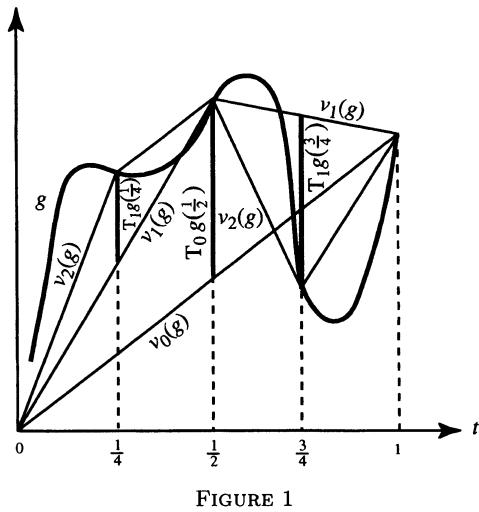
\includegraphics[keepaspectratio]{images/part002_94c2d949.jpg}}

one can then apply Lemma 3 with \(t = \frac{k - 1}{2^n}\) , \(t' = \frac{k}{2^n}\) , whence

\[
\int_ {\Omega} \left| \mathrm{T} _ {n} g \left(\frac {2 k - 1}{2 ^ {n + 1}}\right) \right| ^ {3} d m (g) = \frac {1}{(8 \pi) ^ {1 / 2}} 2 ^ {- \frac {3 n}{2}}.\tag{46}
\]

By (44), we then have

\[
\int_ {\Omega} \| \mathrm{T} _ {n} g \| ^ {3} d m (g) \leqslant \sum_ {k = 1} ^ {2 ^ {n}} \int_ {\Omega} \left| \mathrm{T} _ {n} g \left(\frac {2 k - 1}{2 ^ {n + 1}}\right) \right| ^ {3} d m (g) = \frac {1}{(8 \pi) ^ {1 / 2}} 2 ^ {n} \cdot 2 ^ {- \frac {3 n}{2}},
\]

whence the lemma.

By Lemma 4, the mapping \(\mathbf{T}_n\) of \(\Omega\) into the Banach space \(\mathcal{C}\) belongs to \(\mathrm{L}_{\mathcal{C}}^3 (\Omega ,m)\) and \(\mathrm{N}_3(\mathrm{T}_n)\leqslant \frac{1}{(8\pi)^{1 / 6}} (2^{-1 / 6})^n\) , whence \(\sum_{n = 0}^{\infty}\mathrm{N}_3(\mathrm{T}_n) < + \infty\) . By Prop. 6 of Ch. IV, §3, No.~3, there exists a set \(\Omega_0\subset \Omega\) such that \(\Omega -\Omega_0\) is \(m\) -negligible and such that the series \(\sum_{n = 0}^{\infty}\mathrm{T}_n(g)\) converges absolutely in \(\mathcal{C}\) for every \(g\in \Omega_0\) . One then defines an \(m\) -measurable mapping \(u\) of \(\Omega\) into \(\mathcal{C}\) by

\[
u (g) = \left\{ \begin{array}{c l} \sum_ {n = 0} ^ {\infty} \mathrm{T} _ {n} g = \lim _ {n \to \infty} u _ {n} (g) & \text { for } g \in \Omega_ {0} \\ 0 & \text { for } g \in \Omega - \Omega_ {0}. \end{array} \right.\tag{47}
\]

Since \(u_{n}(g)\) and \(g\) coincide on \(\mathbf{D}_m \subset \mathbf{D}_n\) for \(0 \leqslant m \leqslant n\) , it is immediate that the restriction of \(u(g)\) to \(\mathbf{D}\) is equal to \(g\) for every \(g \in \Omega_0\) .

\begin{enumerate}
\def\labelenumi{\Alph{enumi})}
\setcounter{enumi}{2}
\tightlist
\item
  Construction of a Gaussian measure on \(\mathcal{C}\) :
\end{enumerate}

Let \(w'\) be the bounded measure on \(\mathcal{C}\) that is the image of \(m\) under the \(m\) -measurable mapping \(u: \Omega \to \mathcal{C}\) . We are going to show that \(w'\) is a Gaussian measure on \(\mathcal{C}\) , with variance \(W\) , whence \(w = w'\) . Denote by \(\mathcal{D}\) the linear subspace of \(\mathcal{M}^1\) generated by the measures \(\varepsilon_t\) for \(t\) running over \(D\) .

Lemma 5. --- For every measure \(\mu \in \mathcal{D}\) ,

\[
\int_ {\mathcal {C}} e ^ {i \langle f, \mu \rangle} d w ^ {\prime} (f) = e ^ {- W (\mu) / 2}.\tag{48}
\]

Set \(\mu=c_{1}\varepsilon_{t_{1}}+c_{2}\varepsilon_{t_{2}}+\cdots+c_{n}\varepsilon_{t_{n}}\) with \(t_{1},\ldots,t_{n}\) in D and \(c_{1},\ldots,c_{n}\) in R. For every \(g\in\Omega_{0}\) , the function \(u(g)\) coincides with g on D; therefore

\[
\langle u (g), \mu \rangle = \sum_ {j = 1} ^ {n} c _ {j} g (t _ {j}) \quad (g \in \Omega_ {0}).\tag{49}
\]

Also,

\[
\mathrm{W} (\mu) = \sum_ {j, k = 1} ^ {n} c _ {j} c _ {k} \inf (t _ {j}, t _ {k}),\tag{50}
\]

and, since m is the Gaussian measure on \(\Omega\) with covariance M, and \(\Omega - \Omega_{0}\) is m-negligible, we have

\[
\int_ {\Omega_ {0}} e ^ {i \sum_ {j = 1} ^ {n} c _ {j} g (t _ {j})} d m (g) = \exp \Big (- \frac {1}{2} \sum_ {j, k = 1} ^ {n} c _ {j} c _ {k} \inf (t _ {j}, t _ {k}) \Big).\tag{51}
\]

Now, \(\Omega - \Omega_0\) is \(m\) -negligible and \(w' = u(m)\) ; it follows that

\[
\int_ {\mathcal {C}} e ^ {i \langle f, \mu \rangle} d w ^ {\prime} (f) = \int_ {\Omega_ {0}} e ^ {i \langle u (g), \mu \rangle} d m (g).\tag{52}
\]

The formula (48) follows immediately from the formulas (49) to (52).

Lemma 6. --- Let \(\mu \in \mathcal{M}^1\) . There exists a sequence of measures \(\mu_n \in \mathcal{D}\) such that \(\mu(f) = \lim_{n \to \infty} \mu_n(f)\) for all \(f \in \mathcal{C}\) and \(\mathrm{W}(\mu) = \lim_{n \to \infty} \mathrm{W}(\mu_n)\) .

Let \(I = [0,1]\) . The space \(\mathcal{M}^1\) of bounded measures on \(T = ]0,1]\) will be identified with the subspace of \(\mathcal{M}(I)\) formed by the measures that place no weight at 0. \(^{(3)}\) We equip \(\mathcal{M}(I)\) with the vague topology. The mapping \(t \mapsto \varepsilon_t\) of I into \(\mathcal{M}(I)\) is continuous (Ch. III, §1, No.~9, Prop. 13); since D is dense in I, the closure \(\overline{\mathcal{D}}\) of \(\mathcal{D}\) contains all of the point measures. Let A be the set of measures \(\nu \in \mathcal{D}\) such that \(\| \nu \| \leqslant \| \mu \|\) ; the measure \(\mu\) is in the closure of A (Ch. III, §2, No.~4, Cor. 1 of Th. 1). The set A is relatively compact in \(\mathcal{M}(I)\) (Ch. III, §1, No.~9, Prop. 15) and the compact subsets of \(\mathcal{M}(I)\) are metrizable (TVS, III, §3, No.~4, Cor. 2 of Prop. 6, \(^{(4)}\) and GT, X, §3, No.~3, Th. 1). Therefore there exists a sequence of measures \(\mu_n \in A\) converging to \(\mu\) in \(\mathcal{M}(I)\) . Since \(\mathcal{C}\) is identified with the subspace of continuous functions on I zero at the origin, we have \(\mu(f) = \lim_{n \to \infty} \mu_n(f)\) for all \(f \in \mathcal{C}\) . Moreover, since \(\mathcal{C}(I) \otimes \mathcal{C}(I)\) is dense in the normed space \(\mathcal{C}(I \times I)\) (Ch. III, §4, No.~1, Lemma 1), the relations \(\lim_{n \to \infty} \mu_n = \mu\) and \(\| \mu_n \| \leqslant \| \mu \|\) imply that \(\lim_{n \to \infty} (\mu_n \otimes \mu_n) = \mu \otimes \mu\) (Ch. III, §1, No.~10, Prop. 17); since the measures \(\mu_n\) and \(\mu\) place no weight at 0, we have

\[
\begin{array}{r} \mathrm{W} (\mu_ {n}) = \int_ {\mathrm{I}} \int_ {\mathrm{I}} \inf (t, t ^ {\prime}) d \mu_ {n} (t) d \mu_ {n} (t ^ {\prime}), \\ \mathrm{W} (\mu) = \int_ {\mathrm{I}} \int_ {\mathrm{I}} \inf (t, t ^ {\prime}) d \mu (t) d \mu (t ^ {\prime}), \end{array}
\]

whence \(\lim_{n\to \infty}\mathrm{W}(\mu_n) = \mathrm{W}(\mu)\) .

It remains to prove that the Fourier transform of \(w'\) is equal to \(e^{-\mathbf{W}/2}\) . Let \(\mu \in \mathcal{M}^1\) ; choose measures \(\mu_n \in \mathcal{D}\) as in Lemma 6. The measure \(w'\) is bounded, and \(|e^{i\langle f,\mu_n\rangle}| = 1\) for all \(n\) ; Lemma 5 and Lebesgue's convergence theorem (Ch. IV, §4, No.~3, Th. 2) then imply

\[
\begin{array}{r l} \int_ {\mathcal {C}} e ^ {i \langle f, \mu \rangle} d w ^ {\prime} (f) & = \lim _ {n \to \infty} \int_ {\mathcal {C}} e ^ {i \langle f, \mu_ {n} \rangle} d w ^ {\prime} (f) \\ & = \lim _ {n \to \infty} e ^ {- \mathrm{W} (\mu_ {n}) / 2} = e ^ {- \mathrm{W} (\mu) / 2}. \end{array}\tag{Q.E.D.}
\]

The measure \(w\) on \(\mathcal{C}\) whose Fourier transform is equal to \(e^{-\mathrm{W} / 2}\) is called the Wiener measure on \(\mathcal{C}\) .

Remark. --- For every semi-open interval \(J = ]a, b]\) contained in \(T\) , let us set \(l(J) = b - a\) (the length of \(J\) ) and denote by \(A_J\) the linear form \(f \mapsto f(b) - f(a)\) on \(\mathcal{C}\) . It can be shown that the Wiener measure is characterized by the following property:

Let \(J_{1},\ldots,J_{n}\) be semi-open intervals contained in T and pairwise disjoint. The image of the measure w under the linear mapping \(f\mapsto\left(\mathrm{A}_{\mathrm{J}_{1}}(f),\ldots,\mathrm{A}_{\mathrm{J}_{n}}(f)\right)\) of C into \(R^{n}\) is equal to \(\gamma_{a_{1}}\otimes\cdots\otimes\gamma_{a_{n}}\) with \(a_{i}=l(J_{i})^{1/2}\) for \(1\leqslant i\leqslant n\) .

\subsection{Continuity of the Fourier transform}

PROPOSITION 8. --- Let E be a locally convex space, \(\mu\) a promeasure on E, and \(\Phi\) the Fourier transform of \(\mu\) . One has the inequalities

\[
\left| \Phi (x ^ {\prime}) \right| \leqslant \Phi (0)\tag{53}
\]

\[
\left| \Phi (x ^ {\prime}) - \Phi (y ^ {\prime}) \right| ^ {2} \leqslant 2 \Phi (0) \big (\Phi (0) - \mathcal {R} \Phi (x ^ {\prime} - y ^ {\prime}) \big)\tag{54}
\]

for \(x', y'\) in \(\mathbf{E}'\) .

Formula (5) of No.~3 permits reducing to the case that E is finite-dimensional and \(\mu\) is a measure. Then

\[
\left| \Phi (x ^ {\prime}) \right| = \left| \int_ {\mathrm{E}} e ^ {i \langle x, x ^ {\prime} \rangle} d \mu (x) \right| \leqslant \int_ {\mathrm{E}} | e ^ {i \langle x, x ^ {\prime} \rangle} | d \mu (x) = \int_ {\mathrm{E}} d \mu (x) = \Phi (0),
\]

whence (53). Moreover, if \(a\) and \(b\) are real numbers, then

\[
\left| e ^ {i a} - e ^ {i b} \right| ^ {2} = \left| e ^ {i b} \right| ^ {2} \left| e ^ {i (a - b)} - 1 \right| ^ {2} = \left(e ^ {i (a - b)} - 1\right) \left(e ^ {- i (a - b)} - 1\right) = 2 - 2 \cos (a - b);
\]

by the Cauchy--Schwarz inequality, we then have

\[
\begin{array}{r l} \big | \Phi (x ^ {\prime}) - \Phi (y ^ {\prime}) \big | ^ {2} & = \Big | \int_ {\mathrm{E}} \big (e ^ {i \langle x, x ^ {\prime} \rangle} - e ^ {i \langle x, y ^ {\prime} \rangle} \big) d \mu (x) \Big | ^ {2} \\ & \leqslant \int_ {\mathrm{E}} \big | e ^ {i \langle x, x ^ {\prime} \rangle} - e ^ {i \langle x, y ^ {\prime} \rangle} \big | ^ {2} d \mu (x) \int_ {\mathrm{E}} 1 ^ {2} d \mu (x) \\ & = \int_ {\mathrm{E}} (2 - 2 \cos \langle x, x ^ {\prime} - y ^ {\prime} \rangle) d \mu (x) \cdot \Phi (0) \\ & = 2 \Phi (0) \big (\Phi (0) - \mathcal {R} \Phi (x ^ {\prime} - y ^ {\prime}) \big), \end{array}
\]

whence (54).

COROLLARY. --- Equip E' with a topology compatible with its vector space structure. For \(\Phi\) to be continuous, it is necessary and sufficient that its real part \(\mathcal{R}\Phi\) be continuous at the origin, in which case \(\Phi\) is uniformly continuous.

This follows from the inequality (54).

Let F be a locally convex space. We equip the dual \(F'\) of F with a topology compatible with the duality between F and \(F'\) , and we identify F with the dual of \(F'\) . Consequently, the Fourier transform of a bounded measure \(\mu\) on \(F'\) is the function \(F\mu\) on F defined by

\[
(\mathcal {F} \mu) (x) = \int_ {\mathrm{F} ^ {\prime}} e ^ {i \langle x, x ^ {\prime} \rangle} d \mu (x ^ {\prime}).
\]

PROPOSITION 9. --- If F is barreled, then the Fourier transform of every bounded measure on \(F'\) is a uniformly continuous function on F.

Let \(\mu\) be a bounded measure on \(\mathbf{F}'\) and \(\Phi\) its Fourier transform. Let \(\varepsilon > 0\) . There exists a compact subset \(\mathbf{K}\) of \(\mathbf{F}'\) such that \(\mu(\mathbf{F}' - \mathbf{K}) \leqslant \varepsilon\) . Now, \(\mathbf{K}\) is compact for the weak topology \(\sigma(\mathbf{F}', \mathbf{F})\) , hence is equicontinuous because \(\mathbf{F}\) is barreled (TVS, III, §4, No.~2, Th. 1). Therefore there exists a symmetric neighborhood \(\mathbf{U}\) of \(0\) in \(\mathbf{F}\) whose polar \(\mathbf{U}^{\circ}\) contains \(\mathbf{K}\) . Let \(x\) be in \(\varepsilon \mathrm{U}\) ; then

\[
\Phi (0) - \mathcal {R} \Phi (x) = \int_ {\mathrm{F} ^ {\prime}} \left(1 - \cos \langle x, x ^ {\prime} \rangle\right) d \mu (x ^ {\prime}).
\]

Now, \(0 \leqslant 1 - \cos \langle x, x' \rangle \leqslant 2\) for every \(x' \in \mathbf{F}' - \mathbf{K}\) , and

\[
1 - \cos \langle x, x ^ {\prime} \rangle \leqslant \frac {1}{2} \langle x, x ^ {\prime} \rangle^ {2} \leqslant \frac {\varepsilon^ {2}}{2}
\]

for \(x^{\prime}\in \mathbf{K}\subset \mathbf{U}^{\circ}\) ; it follows that

\[
0 \leqslant \Phi (0) - \mathcal {R} \Phi (x) \leqslant 2 \mu (\mathrm{F} ^ {\prime} - \mathrm{K}) + \frac {\varepsilon^ {2}}{2} \mu (\mathrm{K}) \leqslant 2 \varepsilon + \frac {\varepsilon^ {2}}{2} \mu (\mathrm{F} ^ {\prime}).
\]

The second member of this inequality tends to 0 with \(\varepsilon\) ; thus \(\mathcal{R}\Phi\) is continuous at 0 and the proposition follows from the Cor. of Prop. 8.

\subsection{Minlos's lemma}

Let T be a finite-dimensional vector space and \(\mu\) a bounded measure on \(T'\) ; we shall identify T with the dual of \(T'\) , so that the Fourier transform \(\Phi\) of \(\mu\) is a function on T. We assume given two positive quadratic forms h and q on T and a number \(\varepsilon > 0\) . For every real number r > 0, we denote by \(C_{r}\) the set of \(x' \in T'\) such that \(\langle x, x' \rangle^{2} \leqslant r^{2} h(x)\) for all \(x \in T\) .

PROPOSITION 10. --- Under the hypothesis \(\Phi(0) - \mathcal{R}\Phi \leqslant \varepsilon + q\) , we have

\[
\mu (\mathrm{T} ^ {\prime} - \mathrm{C} _ {r}) \leqslant 3 \left(\varepsilon + r ^ {- 2} \operatorname{Tr} (q / h)\right)\tag{55}
\]

for every \(r > 0\) .

One writes \(\operatorname{Tr}(q/h)\) for the trace of q with respect to h (cf.~Annex, No.~1). The formula (55) is trivial when \(\operatorname{Tr}(q/h)\) is infinite. We assume henceforth that \(\operatorname{Tr}(q/h)\) is finite, hence that \(h(x)=0\) implies \(q(x)=0\) for \(x\in T\) .

Let \(a_1, \ldots, a_n\) be elements of \(\mathbf{T}\) , and \(\mathbf{D}\) the set of \(x' \in \mathbf{T}'\) such that \(\sum_{j=1}^{n} \langle a_j, x' \rangle^2 > 1\) . For every real \(t \geqslant 0\) we have \(3(1 - e^{-t/2}) \geqslant 0\) , and we even have

\[
3 (1 - e ^ {- t / 2}) \geqslant 3 (1 - e ^ {- 1 / 2}) \geqslant 3 \left(1 - \left(\frac {9}{4}\right) ^ {- 1 / 2}\right) = 1
\]

for \(t > 1\) , because \(e > \frac{9}{4}\) . Applying these inequalities to \(t = \sum_{j=1}^{n} \langle a_j, x' \rangle^2\) , we obtain

\[
\mu (\mathrm{D}) \leqslant 3 \int_ {\mathrm{T} ^ {\prime}} \left(1 - \exp \left(- \frac {1}{2} \sum_ {j = 1} ^ {n} \langle a _ {j}, x ^ {\prime} \rangle^ {2}\right)\right) d \mu (x ^ {\prime}).\tag{56}
\]

Let \(\gamma\) be the measure on \(\mathbf{R}\) having density \(t \mapsto (2\pi)^{-1/2} e^{-t^2/2}\) with respect to Lebesgue measure. By Lemma 2 of No.~4,

\[
\int_ {\mathbf {R}} e ^ {i u t} d \gamma (t) = e ^ {- u ^ {2} / 2}
\]

for all real \(u\) . Consequently,

\[
\begin{array}{l} 1 - \exp \left(- \frac {1}{2} \sum_ {j = 1} ^ {n} \langle a _ {j}, x ^ {\prime} \rangle^ {2}\right) \\ = \int \dots \int \left(1 - e ^ {i \sum_ {j = 1} ^ {n} \langle a _ {j}, x ^ {\prime} \rangle t _ {j}}\right) d \gamma (t _ {1}) \dots d \gamma (t _ {n}) \end{array}\tag{57}
\]

for all \(x' \in T'\) . The function of \(x', t_{1}, \ldots, t_{n}\) to be integrated in the second member is continuous and is bounded above in absolute value by 2, and the measures \(\mu\) and \(\gamma\) are bounded; one can therefore integrate the two members of (57) with respect to \(d\mu(x')\) and interchange the integrations with respect to \(\mu\) and \(\gamma\) ; one obtains

\[
\begin{array}{l} \int_ {\mathbf {T} ^ {\prime}} \left(1 - \exp \left(- \frac {1}{2} \sum_ {j = 1} ^ {n} \langle a _ {j}, x ^ {\prime} \rangle^ {2}\right)\right) d \mu (x ^ {\prime}) \\ = \int \dots \int \left(\Phi (0) - \Phi \left(\sum_ {j = 1} ^ {n} t _ {j} a _ {j}\right)\right) d \gamma (t _ {1}) \dots d \gamma (t _ {n}). \end{array}\tag{58}
\]

Since \(q\) is a quadratic form on \(\mathbf{T}\) , there exist real numbers \(q_{jk}\) such that

\[
q \left(\sum_ {j = 1} ^ {n} t _ {j} a _ {j}\right) = \sum_ {j, k} q _ {j k} t _ {j} t _ {k}
\]

for \(t_1, \ldots, t_n\) real; in particular, \(q_{jj} = q(a_j)\) for \(1 \leqslant j \leqslant n\) . Moreover, the integral \(\int_{\mathbf{R}} t^n d\gamma(t)\) has the values 1, 0, 1 for \(n = 0, 1, 2\) , respectively (No.~4, Lemma 1). From this, one deduces immediately

\[
\int \dots \int \left(\varepsilon + q \left(\sum_ {j = 1} ^ {n} t _ {j} a _ {j}\right)\right) d \gamma (t _ {1}) \dots d \gamma (t _ {n}) = \varepsilon + \sum_ {j = 1} ^ {n} q (a _ {j}).\tag{59}
\]

Now, the first member of (58) and \(\Phi(0)\) are real numbers; one can therefore replace \(\Phi\) by \(R\Phi\) in the second member of (58). The inequality \(\Phi(0)-\mathcal{R}\Phi\leqslant\varepsilon+q\) and the formulas (56), (58) and (59) then imply

\[
\mu (\mathrm{D}) \leqslant 3 \left(\varepsilon + \sum_ {j = 1} ^ {n} q (a _ {j})\right).\tag{60}
\]

Let us fix the number \(r > 0\) . Since the quadratic form \(h\) is positive, there exist a basis \((e_1, \ldots, e_n)\) of \(T\) and an integer \(m\) between 0 and \(n\) such that

\[
h \left(\sum_ {j = 1} ^ {n} t _ {j} e _ {j}\right) = \sum_ {j = 1} ^ {m} t _ {j} ^ {2}
\]

for \(t_1, \ldots, t_n\) real (Annex, No.~1, Prop. 2). It is then immediate that \(\mathbf{C}_r\) consists of the \(x' \in \mathbf{T}'\) such that

\[
\sum_ {j = 1} ^ {m} \langle e _ {j}, x ^ {\prime} \rangle^ {2} \leqslant r ^ {2}, \quad \sum_ {j = m + 1} ^ {n} \langle e _ {j}, x ^ {\prime} \rangle^ {2} = 0.
\]

For every integer \(l \geqslant 1\) , let \(D_l\) be the set of \(x' \in T'\) satisfying the inequality

\[
\sum_ {j = 1} ^ {m} \left\langle r ^ {- 1} e _ {j}, x ^ {\prime} \right\rangle^ {2} + \sum_ {j = m + 1} ^ {n} \left\langle l e _ {j}, x ^ {\prime} \right\rangle^ {2} > 1.
\]

One sees easily that the sequence \((\mathrm{D}_l)_{l\geqslant 1}\) is increasing with union \(\mathbf{T}' - \mathbf{C}_r\), whence

\[
\mu (\mathrm{T} ^ {\prime} - \mathrm{C} _ {r}) = \lim _ {l \to \infty} \mu (\mathrm{D} _ {l}).\tag{61}
\]

But by (60),

\[
\mu \left(\mathrm{D} _ {l}\right) \leqslant 3 \left(\varepsilon + \sum_ {j = 1} ^ {m} r ^ {- 2} q \left(e _ {j}\right) + \sum_ {j = m + 1} ^ {n} l ^ {2} q \left(e _ {j}\right)\right);\tag{62}
\]

for \(j = m + 1, \ldots, n\) we have \(h(e_j) = 0\) , therefore \(q(e_j) = 0\) . Moreover, \(\operatorname{Tr}(q/h) = \sum_{j=1}^{m} q(e_j)\) (Annex, No.~1, Prop. 2). The relation (55) then follows from (61) and (62).

Q.E.D.

\subsection{Measures on the dual of a nuclear space}

Let F be a locally convex space. Let \(T_{s}\) be the weak topology \(\sigma(\mathbf{F}^{\prime},\mathbf{F})\) on \(F^{\prime}\) , and \(T_{c}\) the topology of uniform convergence on the compact convex subsets of F. By Mackey's theorem (TVS, IV, §1, No.~1, Th. 1) the topologies \(T_{s}\) and \(T_{c}\) on \(F^{\prime}\) are compatible with the duality between F and \(F^{\prime}\) ; the same is therefore true of every locally convex topology T on \(F^{\prime}\) intermediate to \(T_{s}\) and \(T_{c}\) . If T is such a topology, and \(F^{\prime}_{T}\) denotes the space \(F^{\prime}\) equipped with T, we shall identify F with the dual of \(F^{\prime}_{T}\) . The promeasures on \(F^{\prime}\) are therefore the same for all topologies T of the preceding type, and if \(\mu\) is such a promeasure then its Fourier transform is a function on F.

One calls Sazonov's topology on F the locally convex topology S defined by the continuous seminorms N satisfying the following condition: \(N^{2}\) is a positive quadratic form on F and there exists a continuous positive quadratic form H on F such that \(\operatorname{Tr}\left(\mathrm{N}^{2}/\mathrm{H}\right)<+\infty\) . The topology S is coarser than the given topology on F; if these topologies are identical, F is said to be nuclear. This class of spaces will be studied in detail later on.

THEOREM 2 (Minlos). --- Let F be a locally convex space, T a locally convex topology on \(F'\) intermediate to \(T_{s}\) and \(T_{c}\) , and \(\mu\) a promeasure on \(F'_{T}\) . Assume that the Fourier transform \(\Phi\) of \(\mu\) is continuous on F for the Sazonov topology. Then \(\mu\) is a measure on \(F'_{T}\) .

Let \(\varepsilon > 0\) . Since \(\Phi\) is continuous for the Sazonov topology on \(F\) , there exist two continuous positive quadratic forms \(Q\) and \(H\) on \(F\) such that \(\operatorname{Tr}(Q / H) < +\infty\) and

\[
\Phi (0) - \mathcal {R} \Phi (x) \leqslant \varepsilon / 6
\]

for every \(x \in \mathbf{F}\) such that \(\mathbf{Q}(x) \leqslant 1\) . By Prop. 8 of No.~8, \(|\mathcal{R}\Phi(x)| \leqslant \Phi(0)\) for all \(x \in \mathbf{F}\) , whence

\[
\Phi (0) - \mathcal {R} \Phi (x) \leqslant \varepsilon / 6 + 2 \Phi (0) \mathrm{Q} (x)\tag{63}
\]

for all \(x \in \mathbf{F}\) .

Set \(r = \left(12\Phi(0)\mathrm{Tr}(\mathbf{Q}/\mathbf{H})\varepsilon^{-1}\right)^{1/2}\) and denote by \(K\) the set of \(x' \in F_{\mathcal{T}}'\) such that \(\langle x, x' \rangle^2 \leqslant r^2\mathrm{H}(x)\) for all \(x \in F\) . Since \(H^{1/2}\) is a continuous semi-norm on \(F\) , the set \(K\) is equicontinuous and closed in \(F_{\mathcal{T}}'\) ; it is therefore compact in \(F_{\mathcal{T}}'\) by Ascoli's theorem (GT, X, §2, No.~5, Cor. 1 of Th. 2).

Let V be a closed linear subspace of \(F'_{T}\) with finite codimension; then, V is the orthogonal of a finite-dimensional linear subspace T of F. Let \(\mu_{V}\) be the measure on \(T'\) that is the image of the promeasure \(\mu\) on \(F'_{T}\) under the mapping \(p_{V}\) that is the transpose of the canonical injection of T into F; its Fourier transform is the restriction of \(\Phi\) to T. Finally, by the Hahn--Banach theorem (TVS, II, §3, No.~2, Cor. 1 of Th. 1), \(p_{\mathrm{V}}(\mathrm{K})\) is equal to the set \(C_{r}\) of \(x' \in T'\) such that \(\langle x, x' \rangle^{2} \leqslant r^{2}\mathrm{H}(x)\) for all \(x \in T\) . By the inequality (63), one can apply Prop. 10 of No.~9 to the measure \(\mu_{V}\) on \(T'\) , on taking for q the restriction of \(2\Phi(0)\mathrm{Q}\) to T and for h that of H. Then \(\mathrm{Tr}(q/h) \leqslant 2\Phi(0)\operatorname{Tr}(\mathrm{Q}/\mathrm{H})\) , whence

\[
\mu_ {\mathrm{V}} \left(\mathrm{T} ^ {\prime} - \mathrm{C} _ {r}\right) \leqslant 3 \left(\frac {\varepsilon}{6} + 2 \Phi (0) \operatorname{Tr} (\mathrm{Q} / \mathrm{H}) r ^ {- 2}\right) = \varepsilon .
\]

Since \(p_V\) defines, by passage to the quotient, an isomorphism of \(F_{\mathcal{T}}' / V\) onto \(T'\) , Prop. 1 of No.~1 then shows that \(\mu\) is a measure on \(F_{\mathcal{T}}'\) .

Q.E.D.

COROLLARY. --- Let F be a barreled nuclear space, T a locally convex topology on \(F'\) intermediate to \(T_{s}\) and \(T_{c}\) , \(\mu\) a promeasure on \(F'_{T}\) , and \(\Phi\) the Fourier transform of \(\mu\) . For \(\mu\) to be a measure, it is necessary and sufficient that \(\Phi\) be continuous on F.

Necessity follows from Prop. 9 of No.~8 and sufficiency from Th. 2.

Remark. --- Let F be a barreled space and T a locally convex topology on \(F'\) intermediate to \(T_s\) and \(T_c\) . Every subset of \(F'\) compact for T is compact for the coarser topology \(T_s\) . Conversely, let K be a subset of \(F'\) compact for \(T_s\) . Since F is barreled, K is equicontinuous (TVS, III, §4, No.~2, Th. 1); but by Ascoli's theorem, every equicontinuous subset of \(F'\) is relatively compact for \(T_c\) and a fortiori for T, therefore K is contained in a subset of \(F'\) compact for T. It is not difficult to infer from this that the identity mapping of \(F'_T\) onto \(F'_{T_s}\) defines a bijection between the sets of measures on these two spaces.

\subsection{Measures on a Hilbert space}

Let E be a real Hilbert space, in which the scalar product is denoted \((x|y)\) . There exists an isomorphism j of E onto its dual \(E'\) , characterized by the formula \(\langle x,j(y)\rangle=(x|y)\) for x,y in E (TVS, V, §1, No.~7, Th. 3). We will identify E and \(E'\) by means of j. The Fourier transform of a promeasure \(\mu\) on E is therefore a function \(\mathcal{F}\mu\) on E; when \(\mu\) is a

measure, we have

\[
(\mathcal {F} \mu) (x) = \int_ {\mathrm{E}} e ^ {i (x | y)} d \mu (y) \quad (x \in \mathrm{E}).\tag{64}
\]

THEOREM 3 (Prokhorov--Sazonov) --- Let E be a Hilbert space and \(E_{s}\) the space E equipped with the weakened topology. Let \(\mu\) be a promeasure on E, and \(\Phi\) its Fourier transform. The following conditions are equivalent:

\begin{enumerate}
\def\labelenumi{\alph{enumi})}
\item
  The function \(\Phi\) is continuous on \(\mathbf{E}\) for the Sazonov topology.
\item
  For every \(\varepsilon > 0\) , there exists a nuclear positive quadratic form \(\mathbb{Q}\) on \(\mathbf{E}\) such that \(\Phi(0) - \mathcal{R}\Phi \leqslant \varepsilon + \mathbb{Q}\) .
\item
  The promeasure \(\mu\) is a measure on \(\mathbf{E}_s\) .
\end{enumerate}

\(b) \Rightarrow a)\) : This follows from Prop. 8 of No.~8 (cf.~the inequality (54)).

\(a) \Rightarrow c)\) : This follows from Theorem 2 of No.~10.

\(c) \Rightarrow b)\) : Suppose that \(\mu\) is a measure on \(\mathbf{E}_s\) . Let \(\varepsilon > 0\) . For every integer \(n \geqslant 1\) , the set \(\mathrm{B}_n\) of \(x \in \mathbf{E}\) with norm \(\leqslant n\) is a closed subset of \(\mathbf{E}_s\) , and \(\mathbf{E} = \bigcup_{n \geqslant 1} \mathrm{B}_n\) . Therefore there exists an integer \(n \geqslant 1\) such that

\(\mu (\mathbf{E} - \mathbf{B}_n) <   \frac{\varepsilon}{2}.\) The formula

\[
\mathrm{Q} (x) = \frac {1}{2} \int_ {\mathrm{B} _ {n}} (x | y) ^ {2} d \mu (y)\tag{65}
\]

defines a positive quadratic form \(\mathbf{Q}\) on \(\mathbf{E}\) . Set \(\mathrm{C} = \frac{n^2}{2}\mu (\mathrm{B}_n)\) . If \((e_1,\ldots ,e_p)\) is a finite orthonormal sequence in \(\mathbf{E}\) , then

\[
\sum_ {j = 1} ^ {p} (e _ {j} | y) ^ {2} \leqslant \| y \| ^ {2} \leqslant n ^ {2}
\]

for every \(y \in \mathbf{B}_n\) by Bessel's inequality. It follows by integration that

\[
\sum_ {j = 1} ^ {p} \mathrm{Q} (e _ {j}) = \frac {1}{2} \int_ {\mathrm{B} _ {n}} \sum_ {j = 1} ^ {p} (e _ {j} | y) ^ {2} d \mu (y) \leqslant \frac {n ^ {2}}{2} \mu (\mathrm{B} _ {n}) = \mathrm{C},
\]

therefore Q is nuclear.

Moreover, \(1 - \cos t \leqslant \inf \left(2, \frac{t^2}{2}\right)\) for every real number \(t\) , whence

\[
\begin{array}{r l} \Phi (0) - \mathcal {R} \Phi (x) & = \int_ {\mathrm{E}} \bigl (1 - \cos (x | y) \bigr) d \mu (y) \\ & \leqslant \int_ {\mathrm{B} _ {n}} \frac {1}{2} (x | y) ^ {2} d \mu (y) + \int_ {\mathrm{E} - \mathrm{B} _ {n}} 2 \cdot d \mu (y) \\ & <   \mathrm{Q} (x) + \varepsilon \end{array}
\]

for all \(x \in \mathbf{E}\) . Thus \(b)\) is verified.

Q.E.D.

COROLLARY 1. --- Let \(E_{1}\) and \(E_{2}\) be two Hilbert spaces, u a Hilbert--Schmidt mapping of \(E_{1}\) into \(E_{2}\) , and \(\mu\) a promeasure on \(E_{1}\) . Assume that the Fourier transform \(\Phi\) of \(\mu\) is continuous on \(E_{1}\) . Then the promeasure \(\nu = u(\mu)\) is a measure on \(E_{2}\) equipped with the weak topology.

With the identifications of \(E_{1}\) and \(E_{2}\) with their duals introduced in this No., the Fourier transform of \(\nu\) is equal to \(\Phi\circ u^{*}\) , where \(u^{*}\) is the adjoint of u. Now, \(u^{*}\) is a Hilbert--Schmidt mapping of \(E_{2}\) into \(E_{1}\) (Annex, No.~2), and the quadratic form \(y\mapsto\|u^{*}(y)\|^{2}\) on \(E_{2}\) is therefore nuclear. If \((\mathrm{E}_{2})_{\mathcal{S}}\) denotes \(E_{2}\) equipped with the Sazonov topology, \(u^{*}\) is therefore a continuous linear mapping of \((\mathrm{E}_{2})_{\mathcal{S}}\) into \(E_{1}\) , and \(\Phi_{\nu}=\Phi\circ u^{*}\) is continuous on \((\mathrm{E}_{2})_{\mathcal{S}}\) ; Theorem 3 then shows that \(\nu\) is a measure on the space \(E_{2}\) equipped with the weak topology.

COROLLARY 2. --- Let Q be a nuclear positive quadratic form on the Hilbert space E. The Gaussian promeasure \(\Gamma_{Q}\) on E with variance Q is a measure on \(E_{s}\) .

The Fourier transform \(\Phi\) of \(\Gamma_{Q}\) is equal to \(e^{-\mathbb{Q} / 2}\) . Now, \(e^t \geqslant 1 + t\) for every real number \(t\) , whence \(\Phi(0) - \mathcal{R}\Phi \leqslant \mathbb{Q} / 2\) . The condition \(b)\) of Theorem 3 is therefore verified and \(\Gamma_{Q}\) is a measure on \(\mathbf{E}_s\) .

\subsection{Relations with functions of positive type}

\begin{enumerate}
\def\labelenumi{(\arabic{enumi})}
\setcounter{enumi}{65}
\tightlist
\item
\end{enumerate}

PROPOSITION 11. --- Let E be a finite-dimensional vector space, \(\mu\) a bounded (positive) measure on E, and \(\Phi\) the Fourier transform of \(\mu\) . The function \(\Phi\) is continuous and of positive type on \(E'\) .

The continuity of \(\Phi\) follows from Prop. 9 of No.~8.

Let us show that \(\Phi\) is of positive type. Let \(x_1', \ldots, x_p'\) be in E' and \(c_1, \ldots, c_p\) complex numbers. Then

\[
\begin{array}{r l} \sum_ {j, k} c _ {j} \overline {{{c}}} _ {k} \Phi (x _ {j} ^ {\prime} - x _ {k} ^ {\prime}) & = \int_ {\mathrm{E}} \sum_ {j, k} c _ {j} \overline {{{c}}} _ {k} e ^ {i \langle x, x _ {j} ^ {\prime} - x _ {k} ^ {\prime} \rangle} d \mu (x) \\ & = \int_ {\mathrm{E}} \left| \sum_ {j = 1} ^ {p} c _ {j} e ^ {i \langle x, x _ {j} ^ {\prime} \rangle} \right| ^ {2} d \mu (x) \geqslant 0. \end{array}\tag{Q.E.D.}
\]

One can prove a converse known as Bochner's theorem: every continuous function on \(E'\) of positive type is the Fourier transform of a bounded (positive) measure. \(^{*}\) We shall assume this result for the rest of No.~12.

THEOREM 4. --- Let E be a locally convex space. The Fourier transformation is a bijection of the set of promeasures on E onto the set of functions of positive type on E' whose restriction to every finite-dimensional subspace is continuous.

We know (No.~3, Prop. 3) that the Fourier transformation is injective. Let \(\mu = (\mu_{\mathrm{V}})_{\mathrm{V}\in \mathcal{F}(\mathbf{E})}\) be a promeasure on \(\mathbf{E}\) and \(\Phi\) its Fourier transform. Let \(\mathbf{T}\) be a finite-dimensional subspace of \(\mathbf{E}'\) and let \(\mathbf{V}\) be the orthogonal of \(\mathbf{T}\) in \(\mathbf{E}\) . One can identify \(\mathbf{T}\) with the dual of \(\mathbf{E} / \mathbf{V}\) ; the restriction \(\Phi_{\mathrm{T}}\) of \(\Phi\) to \(\mathbf{T}\) is the Fourier transform of the bounded measure \(\mu_{\mathrm{V}}\) on \(\mathbf{E} / \mathbf{V}\) . By Prop. 11, \(\Phi_{\mathrm{T}}\) is continuous and of positive type on \(\mathbf{T}\) . Since \(\mathbf{T}\) is arbitrary, it is clear that \(\Phi\) is of positive type on \(\mathbf{E}'\) .

Conversely, let \(\Phi\) be a function of positive type on \(\mathbf{E}'\) whose restriction to every finite-dimensional subspace of \(\mathbf{E}'\) is continuous. For every \(V \in \mathcal{F}(\mathbf{E})\) , we identify the dual of \(E/V\) with the orthogonal \(V^{\circ}\) of \(V\) in \(\mathbf{E}'\) ; the restriction \(\Phi_V\) of \(\Phi\) to \(V^{\circ}\) is continuous and of positive type and so, by Bochner's theorem, there exists a bounded (positive) measure \(\mu_V\) on \(E/V\) whose Fourier transform is \(\Phi_V\) . Let \(V\) and \(W\) in \(\mathcal{F}(\mathbf{E})\) be such that \(W \subset V\) , and let \(p_{\mathrm{VW}}\) be the canonical mapping of \(E/W\) onto \(E/V\) ; with the identifications made, \(^{t}p_{\mathrm{VW}}\) is the injection of \(V^{\circ}\) into \(W^{\circ}\) . By formula (4) of No.~3, we then have

\[
\mathcal {F} \big (p _ {\mathrm{VW}} (\mu_ {\mathrm{W}}) \big) = \big (\mathcal {F} \mu_ {\mathrm{W}} \big) \circ {} ^ {t} p _ {\mathrm{VW}} = \Phi_ {\mathrm{W}} \circ {} ^ {t} p _ {\mathrm{VW}} = \Phi_ {\mathrm{V}} = \mathcal {F} \mu_ {\mathrm{V}},
\]

whence \(p_{\mathrm{VW}}(\mu_{\mathrm{W}}) = \mu_{\mathrm{V}}\) by Prop. 3 of No.~3. Consequently, the family \(\mu = (\mu_{\mathrm{V}})_{\mathrm{V} \in \mathcal{F}(\mathrm{E})}\) is a promeasure on E; it is clear that \(\Phi\) is the Fourier transform of \(\mu\) .

COROLLARY. --- Let F be a barreled nuclear space; equip \(F'\) with a locally convex topology T intermediate to the weak topology \(\sigma(\mathbf{F}',\mathbf{F})\) and the topology of uniform convergence on the compact convex subsets of F. The Fourier transformation is a bijection of the set of bounded (positive) measures on \(F'\) onto the set of continuous functions of positive type on F.

This follows immediately from Theorem 4 and the Cor. of Th. 2 of No.~10.*

\specsection{Annex: Complements on Hilbert spaces}

\annexsubsection{\texorpdfstring{Trace of a quadratic form with respect to another \(^{(1)}\)}{Trace of a quadratic form with respect to another (1)}}

In this No., we denote by E a real vector space and by Q, H two positive quadratic forms on E. There exist two symmetric bilinear forms \((x,y)\mapsto(x|y)_{\mathbf{Q}}\) and \((x,y)\mapsto(x|y)_{\mathbf{H}}\) characterized by

\[
\mathrm{Q} (x) = (x | x) _ {\mathrm{Q}}, \quad \mathrm{H} (x) = (x | x) _ {\mathrm{H}}
\]

for all \(x \in E\) .

One calls trace of Q with respect to H and one denotes by \(\operatorname{Tr}\left(\mathbf{Q}/\mathbf{H}\right)\) the positive real number, finite or not, defined as follows:

\begin{enumerate}
\def\labelenumi{\alph{enumi})}
\item
  If there exists an \(x \in \mathbf{E}\) such that \(\mathrm{H}(x) = 0\) and \(\mathrm{Q}(x) \neq 0\) , one sets \(\operatorname{Tr}(\mathrm{Q} / \mathrm{H}) = +\infty\) .
\item
  In the contrary case, \(\operatorname{Tr}(\mathbf{Q}/\mathbf{H})\) is the supremum of the set of numbers of the form \(\sum_{i=1}^{p} \mathbf{Q}(e_i)\) , where \((e_1, \ldots, e_p)\) runs over the set of finite sequences of elements of E orthonormal for H.
\end{enumerate}

Let E be a real Hilbert space and Q a positive quadratic form on E. Set \(\mathrm{H}(x)=\|x\|^{2}\) for all \(x\in E\) ; then H is a positive quadratic form on E. One says that Q is nuclear if \(\mathrm{Tr}\left(\mathrm{Q}/\mathrm{H}\right)\) is finite. For every \(x\in E\) of norm 1, one has \(\mathrm{Q}(x)\leqslant\mathrm{Tr}\left(\mathrm{Q}/\mathrm{H}\right)\) , whence \(Q\leqslant\mathrm{Tr}\left(\mathrm{Q}/\mathrm{H}\right)\cdot\mathrm{H}\) ; in particular, every nuclear form Q is continuous.

Remarks. --- 1) For every subspace F of E, denote by \(Q_{F}\) the restriction of Q to F, and by \(H_{F}\) that of H. Then \(\mathrm{Tr}\left(\mathrm{Q}_{\mathrm{F}}/\mathrm{H}_{\mathrm{F}}\right) \leqslant \mathrm{Tr}\left(\mathrm{Q}/\mathrm{H}\right)\) and \(\mathrm{Tr}\left(\mathrm{Q}/\mathrm{H}\right)\) is the supremum of the numbers \(\mathrm{Tr}\left(\mathrm{Q}_{\mathrm{F}}/\mathrm{H}_{\mathrm{F}}\right)\) for \(F \subset E\) finite-dimensional.

\begin{enumerate}
\def\labelenumi{\arabic{enumi})}
\setcounter{enumi}{1}
\tightlist
\item
  Let \(\mathbf{E}_1\) be a real vector space, \(\mathbf{Q}_1\) and \(\mathbf{H}_1\) two positive quadratic forms on \(\mathbf{E}_1\) , and \(\pi: \mathbf{E} \to \mathbf{E}_1\) a surjective linear mapping. If \(\mathbf{Q} = \mathbf{Q}_1 \circ \pi\) and \(\mathbf{H} = \mathbf{H}_1 \circ \pi\) , then \(\operatorname{Tr}(\mathbf{Q} / \mathbf{H}) = \operatorname{Tr}(\mathbf{Q}_1 / \mathbf{H}_1)\) .
\end{enumerate}

PROPOSITION 1. --- Assume that E is finite-dimensional and H is nondegenerate.

\begin{enumerate}
\def\labelenumi{\alph{enumi})}
\item
  There exists an endomorphism \(u\) of \(\mathbf{E}\) characterized by \((x|y)_{\mathbb{Q}} = (u(x)|y)_{\mathbb{H}}\) for \(x, y\) in \(\mathbf{E}\) .
\item
  \(\operatorname{Tr}(\mathbf{Q} / \mathbf{H}) = \operatorname{Tr}(u)\) .
\item
  \(\operatorname{Tr}(\mathbf{Q} / \mathbf{H}) = \sum_{i=1}^{m} \mathbf{Q}(e_i)\) for every basis \((e_1, \ldots, e_m)\) of E orthonormal for H.
\end{enumerate}

a) follows from the fact that the bilinear form \((x,y)\mapsto (x|y)_{\mathrm{H}}\) is nondegenerate. Every sequence in E orthonormal for H may be completed to a basis of E orthonormal for H. Consequently, \(\operatorname {Tr}(\mathbf{Q} / \mathbf{H})\) is the supremum of the set of numbers of the form \(\sum_{i = 1}^{m}\mathbf{Q}(e_i)\) over all bases \((e_1,\ldots ,e_m)\) of E orthonormal for H. To prove b) and c), it suffices to show that \(\sum_{i = 1}^{m}\mathbf{Q}(e_i) =\) \(\operatorname {Tr}(u)\) for every basis of this kind. Set \(a_{ij} = (u(e_i)|e_j)_{\mathrm{H}} = (e_i|e_j)_{\mathrm{Q}}\) for \(1\leqslant i,j\leqslant m\) ; then \(u(e_i) = \sum_{j = 1}^{m}a_{ij}e_j\) for \(1\leqslant i\leqslant m\) , whence

\[
\operatorname{Tr} (u) = \sum_ {i = 1} ^ {m} a _ {i i} = \sum_ {i = 1} ^ {m} \left(e _ {i} \mid e _ {i}\right) _ {\mathrm{Q}} = \sum_ {i = 1} ^ {m} Q \left(e _ {i}\right).\tag{Q.E.D.}
\]

PROPOSITION 2. --- Assume that E is finite-dimensional. There exist a basis \((e_{1},\ldots,e_{n})\) of E and an integer m with \(0\leqslant m\leqslant n\) such that

\[
\mathrm{H} \left(\sum_ {i = 1} ^ {n} t _ {i} e _ {i}\right) = \sum_ {i = 1} ^ {m} t _ {i} ^ {2}\tag{1}
\]

for \(t_1, \ldots, t_n\) real. If, moreover, the relation \(\mathrm{H}(x) = 0\) implies \(\mathrm{Q}(x) = 0\) for \(x \in \mathbf{E}\) , then \(\operatorname{Tr}(\mathrm{Q}/\mathrm{H}) = \sum_{i=1}^{m} \mathrm{Q}(e_i)\) .

There exists a basis \((e_1', \ldots, e_n')\) of E orthogonal for H. One can assume the basis to be indexed in such a way that \(\mathrm{H}(e_i') > 0\) for \(1 \leqslant i \leqslant m\) and \(\mathrm{H}(e_i') = 0\) for \(m < i \leqslant n\) . Then set \(e_i = e_i' / \mathrm{H}(e_i')^{1/2}\) for \(1 \leqslant i \leqslant m\) and \(e_i = e_i'\) for \(m < i \leqslant n\) ; the relation (1) is satisfied.

Let F be the subspace of E generated by \(e_{m+1}^{\prime},\ldots,e_{n}^{\prime}\) ; it is the set of \(x\in E\) such that \(\mathrm{H}(x)=0\) . Denote by \(\pi\) the canonical mapping of E onto \(E_{1}=E/F\) . Since Q and H are zero on F, there exist two positive quadratic forms \(Q_{1}\) and \(H_{1}\) on \(E_{1}\) such that \(Q=Q_{1}\circ\pi\) and \(H=H_{1}\circ\pi\) . Moreover, \((\pi(e_{1}),\ldots,\pi(e_{m}))\) is a basis of \(E_{1}\) orthonormal for \(H_{1}\) , and therefore \(H_{1}\) is nondegenerate.

By Prop. 1 and Remark 2,

\[
\operatorname{Tr} \left(\mathrm{Q} / \mathrm{H}\right) = \operatorname{Tr} \left(\mathrm{Q} _ {1} / \mathrm{H} _ {1}\right) = \sum_ {i = 1} ^ {m} \mathrm{Q} _ {1} \left(\pi (e _ {i})\right) = \sum_ {i = 1} ^ {m} \mathrm{Q} (e _ {i}).\tag{Q.E.D.}
\]

Remark 3). --- Assume E finite-dimensional and H nondegenerate. Let \((e_1, \ldots, e_n)\) be a basis of E. Set \(q = ((e_i | e_j)_Q)_{1 \leqslant i, j \leqslant n}\) and \(h = ((e_i | e_j)_H)_{1 \leqslant i, j \leqslant n}\) . With notations as in Prop. 1, the matrix of \(u\) for the basis \((e_1, \ldots, e_n)\) of E is equal to \(h^{-1}q\) , whence

\[
\operatorname{Tr} \left(\mathrm{Q} / \mathrm{H}\right) = \operatorname{Tr} \left(h ^ {- 1} q\right) = \operatorname{Tr} \left(q h ^ {- 1}\right).\tag{2}
\]

\annexsubsection{\texorpdfstring{Hilbert--Schmidt mappings \(^{(2)}\)}{Hilbert--Schmidt mappings (2)}}

Let E be a real Hilbert space, in which the scalar product is denoted by \((x|y)\) . There exists an isometry \(j_{E}\) of E onto its dual, characterized by the formula

\[
(x | y) = \langle x, j _ {\mathrm{E}} (y) \rangle \quad \text { for } x, y \text { in } \mathrm{E}\tag{3}
\]

(TVS, V, §1, No.~7, Th. 3).

Let \(E_{1}\) and \(E_{2}\) be two real Hilbert spaces and u a continuous linear mapping of \(E_{1}\) into \(E_{2}\) . One calls adjoint of u the continuous linear mapping \(u^{*} = j_{E_{1}}^{-1} \circ {}^{t}u \circ j_{E_{2}}\) of \(E_{2}\) into \(E_{1}\) . The mapping \(u^{*}\) is characterized by the relation

\[
(u (x _ {1}) | x _ {2}) = (x _ {1} | u ^ {*} (x _ {2})) \quad \text { for } x _ {1} \in \mathrm{E} _ {1}, x _ {2} \in \mathrm{E} _ {2}.\tag{4}
\]

If \(v\) is a continuous linear mapping of \(\mathbf{E}_2\) into a Hilbert space \(\mathbf{E}_3\) , one has \((v \circ u)^* = u^* \circ v^*\) .

Let \(E_{1}\) and \(E_{2}\) be two real Hilbert spaces and u a linear mapping of \(E_{1}\) into \(E_{2}\) . One defines two positive quadratic forms H and Q on \(E_{1}\) by the formulas

\[
\mathrm{H} (x) = \| x \| ^ {2}, \quad \mathrm{Q} (x) = \| u (x) \| ^ {2} \qquad (x \in \mathrm{E} _ {1}).
\]

PROPOSITION 3. --- Suppose u is continuous. Let \((e_{i})_{i\in I}\) be an orthonormal basis of \(E_{1}\) and \((f_{j})_{j\in J}\) an orthonormal basis of \(E_{2}\) . Then

\[
\operatorname{Tr} (\mathrm{Q} | \mathrm{H}) = \sum_ {i \in \mathrm{I}} \| u (e _ {i}) \| ^ {2} = \sum_ {j \in \mathrm{J}} \| u ^ {*} (f _ {j}) \| ^ {2} = \sum_ {i \in \mathrm{I}} \sum_ {j \in \mathrm{J}} (u (e _ {i}) | f _ {j}) ^ {2}.
\]

For every \(x \in \mathbf{E}_1\) , we have \(\|x\|^2 = \sum_{i \in \mathbf{I}} (x|e_i)^2\) , and similarly \(\|y\|^2 = \sum_{j \in \mathbf{J}} (y|f_j)^2\) for every \(y \in \mathbf{E}_2\) . Consequently,

\[
\begin{array}{r l} \sum_ {i \in \mathrm{I}} \| u (e _ {i}) \| ^ {2} & = \sum_ {i \in \mathrm{I}} \sum_ {j \in \mathrm{J}} (u (e _ {i}) | f _ {j}) ^ {2} \\ & = \sum_ {j \in \mathrm{J}} \sum_ {i \in \mathrm{I}} (e _ {i} | u ^ {*} (f _ {j})) ^ {2} \\ & = \sum_ {j \in \mathrm{J}} \| u ^ {*} (f _ {j}) \| ^ {2}. \end{array}
\]

In particular, the number \(\sum_{i\in I}\| u(e_i)\|^2\) is independent of the orthonormal basis \((e_i)_{i\in I}\) of \(\mathbf{E}_1\) .

Set \(t = \operatorname{Tr}(\mathbf{Q}|\mathbf{H})\) . For every finite subset \(I'\) of \(I\) , by definition

\[
\sum_ {i \in I ^ {\prime}} \| u (e _ {i}) \| ^ {2} = \sum_ {i \in I ^ {\prime}} Q (e _ {i}) \leqslant t,
\]

whence \(\sum_{i\in I}\| u(e_i)\|^2\leqslant t\) . Let \((e_1',\dots ,e_p')\) be a finite orthonormal sequence in \(\mathbf{E}_1\) . This sequence can be completed to an orthonormal basis \((e_{\alpha}^{\prime})_{\alpha \in A}\) of \(\mathbf{E}_1\) . Then

\[
\sum_ {\alpha = 1} ^ {p} \left\| u (e _ {\alpha} ^ {\prime}) \right\| ^ {2} \leqslant \sum_ {\alpha \in \mathrm{A}} \left\| u (e _ {\alpha} ^ {\prime}) \right\| ^ {2} = \sum_ {i \in \mathrm{I}} \left\| u (e _ {i}) \right\| ^ {2}
\]

and, passing to the supremum over all \((e_1', \ldots, e_p')\) , one obtains the inequality \(t \leqslant \sum_{i \in I} \| u(e_i) \|^2\) . We have thus established the equality \(t = \sum_{i \in I} \| u(e_i) \|^2\) .

Q.E.D.

One says that \(u\) is a Hilbert-Schmidt mapping of \(\mathbf{E}_1\) into \(\mathbf{E}_2\) if the positive quadratic form \(\mathbf{Q}: x \mapsto \| u(x) \|^2\) on \(\mathbf{E}_1\) is nuclear. When this is so, one has \(\mathbf{Q} \leqslant \operatorname{Tr}(\mathbf{Q}/\mathbf{H}) \cdot \mathbf{H}\) , therefore \(u\) is continuous and

\[
\| u \| \leqslant \operatorname{Tr} (\mathrm{Q/H}) ^ {1 / 2}.
\]

Let \(u: \mathbf{E}_1 \to \mathbf{E}_2\) be a continuous linear mapping. By Prop. 3, \(u\) is a Hilbert--Schmidt mapping if and only if there exists an orthonormal basis \((e_i)_{i \in \mathrm{I}}\) of \(\mathbf{E}_1\) such that \(\sum_{i \in \mathrm{I}} \|u(e_i)\|^2 < +\infty\) . When this is so, every orthonormal basis of \(\mathbf{E}_1\) has the same property. Moreover, if \(u\) is a Hilbert--Schmidt mapping, then so is its adjoint \(u^*\) by virtue of the formula \(\sum_{i \in \mathrm{I}} \|u(e_i)\|^2 = \sum_{j \in \mathrm{J}} \|u^*(f_j)\|^2\) (Prop. 3).

\specialchapter{Exercises}

\exercisesection{}

\begin{enumerate}
\def\labelenumi{\arabic{enumi})}
\tightlist
\item
  Let \(\mathbf{T}\) be a set and \(p\) an encumbrance on \(\mathbf{T}\) . For every subset \(\mathbf{A}\) of \(\mathbf{T}\) , set \(p(\mathbf{A}) = p(\varphi_{\mathbf{A}})\) .
\end{enumerate}

\begin{enumerate}
\def\labelenumi{\alph{enumi})}
\item
  \(p(A) \leqslant p(B)\) when A is contained in B.
\item
  For every sequence \((\mathbf{A}_n)\) , finite or not, of subsets of \(\mathbf{T}\) , \(p(\bigcup \mathbf{A}_n) \leqslant \sum p(\mathbf{A}_n)\) .
\item
  For every increasing sequence \((\mathrm{A}_n)_{n\geqslant 1}\) of subsets of T, \(p\big(\bigcup_{n}\mathrm{A}_{n}\big) = \lim_{n\to \infty}p(\mathrm{A}_n)\) .
\end{enumerate}

\begin{enumerate}
\def\labelenumi{\arabic{enumi})}
\setcounter{enumi}{1}
\tightlist
\item
  Let \(\mathbf{T}\) be a set and \(p\) an encumbrance on \(\mathbf{T}\) . A function \(f \in \mathcal{F}_{+}(\mathbf{T})\) (resp. a subset A of \(\mathbf{T}\) ) is said to be \(p\) -negligible if \(p(f) = 0\) (resp. \(p(\mathbf{A}) = 0\) ).
\end{enumerate}

\begin{enumerate}
\def\labelenumi{\alph{enumi})}
\item
  Let \(f\) and \(g\) be in \(\mathcal{F}_{+}(\mathrm{T})\) and let \(t\) be a positive real number such that \(f \leqslant t \cdot g\) . If \(g\) is \(p\) -negligible, then so is \(f\) . The sum and upper envelope of a sequence of \(p\) -negligible functions are \(p\) -negligible.
\item
  Every subset of a \(p\) -negligible set is \(p\) -negligible, as is the union of a sequence (finite or infinite) of \(p\) -negligible sets.
\item
  Let \(f \in \mathcal{F}_+(\mathrm{T})\) . For every finite real number \(a > 0\) , denote by \(\mathbf{T}_a\) the set of \(t \in \mathrm{T}\) such that \(f(t) \geqslant a\) . Show that \(p(\mathbf{T}_a) \leqslant a^{-1} \cdot p(f)\) . From this, deduce that \(f\) is \(p\) -negligible if and only if the set of \(t \in \mathrm{T}\) such that \(f(t) \neq 0\) is \(p\) -negligible.
\item
  Let \(f \in \mathcal{F}_{+}(\mathrm{T})\) . If \(p(f)\) is finite, the set of \(t \in \mathrm{T}\) such that \(f(t)\) is infinite is \(p\) -negligible.
\item
  Let \(f\) and \(g\) be in \(\mathcal{F}_{+}(\mathrm{T})\) . If the set of \(t \in \mathrm{T}\) such that \(f(t) \neq g(t)\) is \(p\) -negligible, then \(p(f) = p(g)\) .
\end{enumerate}

\begin{enumerate}
\def\labelenumi{\arabic{enumi})}
\setcounter{enumi}{2}
\item
  Let \(\mathbf{T}\) be a set and \(p\) an encumbrance on \(\mathbf{T}\) . For every sequence \((f_n)_{n\geqslant 1}\) of elements of \(\mathcal{F}_{+}(\mathbf{T})\) , \(p(\liminf_{n\to \infty}f_n)\leqslant \liminf_{n\to \infty}p(f_n)\) .
\item
  Let \(\mathbf{T}\) be a set, \(\mathbf{M}\) an encumbrance on \(\mathbf{T}\) , \(\mathbf{E}\) a real or complex Banach space, and \(p\) a finite real number such that \(p \geqslant 1\) . Denote by \(\mathcal{F}\) the set of mappings of \(\mathbf{T}\) into \(\mathbf{E}\) , and, for \(f\) in \(\mathcal{F}\) or in \(\mathcal{F}_{+}(\mathbf{T})\) , set \(\mathrm{N}_p(f) = \mathrm{M}(|f|^p)^{1/p}\) .
\end{enumerate}

\begin{enumerate}
\def\labelenumi{\alph{enumi})}
\item
  For every sequence \((f_n)_{n\geqslant 1}\) of elements of \(\mathcal{F}_{+}(\mathrm{T})\) , \(\mathrm{N}_p\left(\sum_{n\geqslant 1}f_n\right)\leqslant \sum_{n\geqslant 1}\mathrm{N}_p(f_n)\)
\item
  Let \(\mathcal{F}^p\) be the set of \(f \in \mathcal{F}\) such that \(\mathrm{N}_p(f)\) is finite. Show that \(\mathcal{F}^p\) is a linear subspace of \(\mathcal{F}\) , and \(\mathrm{N}_p\) is a semi-norm on \(\mathcal{F}^p\) . Show that the set \(\mathcal{N}\) of \(f \in \mathcal{F}^p\) such that \(\mathrm{N}_p(f) = 0\) is equal to the set of \(f \in \mathcal{F}\) that are zero outside an M-negligible set. Show that the normed space \(\mathcal{F}^p / \mathcal{N}\) is complete (cf.~Ch. IV, §3, No.~3).
\end{enumerate}

\begin{enumerate}
\def\labelenumi{\arabic{enumi})}
\setcounter{enumi}{4}
\item
  Let \(\mathbf{T}\) be a set. Denote by \(\mathcal{B}_{+}(\mathbf{T})\) the set of bounded positive real functions on \(\mathbf{T}\) , and by \(p_0\) a mapping of \(\mathcal{B}_{+}(\mathbf{T})\) into the interval \([0, +\infty]\) of \(\overline{\mathbf{R}}\) satisfying the conditions \(a)\) to \(d)\) of Def. 1 of No.~1. For every function \(f \in \mathcal{F}_{+}(\mathbf{T})\) , denote by \(p(f)\) the supremum of the set of numbers \(p_0(f_0)\) , where \(f_0\) runs over the set of bounded functions \(\leqslant f\) . Show that \(p\) is an encumbrance on \(\mathbf{T}\) . Analogous question, with \(\mathcal{B}_{+}(\mathbf{T})\) replaced by the set of (finite) positive real functions on \(\mathbf{T}\) .
\item
  Let \(\mathbf{T}\) be a set, \(\mathcal{I}_{+}\) a subset of \(\mathcal{F}_{+}(\mathrm{T})\) , and \(\mathbf{M}\) a mapping of \(\mathcal{I}_{+}\) into \(\overline{\mathbf{R}}_{+}\) . We make the following hypotheses:
\end{enumerate}

\begin{enumerate}
\def\labelenumi{\alph{enumi})}
\item
  For every \(f \in \mathcal{I}_+\) and every real number \(t \geqslant 0\) , the function \(t \cdot f\) belongs to \(\mathcal{I}_+\) and \(M(t \cdot f) = t \cdot M(f)\) .
\item
  If \(f\) and \(g\) belong to \(\mathcal{I}_+\) , then so do \(f + g\) , \(\sup(f, g)\) and \(\inf(f, g)\) , and one has \(M(f + g) = M(f) + M(g)\) .
\item
  For every increasing sequence \((f_n)_{n\geqslant 1}\) of elements of \(\mathcal{I}_+\) , the function \(f = \sup f_n\) belongs to \(\mathcal{I}_+\) , and \(\mathrm{M}(f) = \lim_{n\to \infty}\mathrm{M}(f_n)\) .
\end{enumerate}

For every function \(f \in \mathcal{F}_{+}(\mathrm{T})\) , we set \(p(f) = \inf_{g \in \mathcal{I}_{+}, g \geqslant f} \mathrm{M}(g)\) . Show that \(p\) is an encumbrance on \(\mathrm{T}\) (cf.~Ch. IV, §1, No.~3). If \(f\) and \(g\) belong to \(\mathcal{F}_{+}(\mathrm{T})\) and if \(\mathrm{A}\) and \(\mathrm{B}\) are subsets of \(\mathrm{T}\) , then \(p(\sup(f, g)) + p(\inf(f, g)) \leqslant p(f) + p(g)\) and \(p(\mathrm{A} \cup \mathrm{B}) + p(\mathrm{A} \cap \mathrm{B}) \leqslant p(\mathrm{A}) + p(\mathrm{B})\) .

\begin{enumerate}
\def\labelenumi{\arabic{enumi})}
\setcounter{enumi}{6}
\tightlist
\item
  On a Lindelöf space every measure, every function and every subset is moderated.
\end{enumerate}

¶ 8) Let us take up again the notations of Exer. 5 of Ch. IV, §1. Recall that \(\mu = \sum_{k=-\infty}^{\infty} \sum_{n=1}^{\infty} n^{-3} \varepsilon_{(1/n,k/n^2)}\) and \(\mu^{*}(D) = +\infty\) . Show that \(\mu^{\bullet}(D) = 0\) ; deduce from this that \(\mu\) is not moderated, even though it is the sum of a series of measures with pairwise disjoint compact supports. Show that there exists a partition \((X_n)_{n \in \mathbb{N}}\) of \(X\) into Borel subsets \(X_n\) such that \(\mu^{\bullet}(X_n)\) is finite for every \(n \in \mathbb{N}\) .

\begin{enumerate}
\def\labelenumi{\arabic{enumi})}
\setcounter{enumi}{8}
\item
  Let \(\mathbf{T}\) be a topological space. If \(\lambda\) and \(\mu\) are two positive measures on \(\mathbf{T}\) such that \(\lambda^{\bullet}(\mathrm{U}) = \mu^{\bullet}(\mathrm{U})\) for every open set \(\mathbf{U}\) in \(\mathbf{T}\) , then \(\lambda = \mu\) (first prove that \(\lambda^{\bullet}(f) = \mu^{\bullet}(f)\) for every lower semi-continuous function \(f \geqslant 0\) on \(\mathbf{T}\) , then that \(\lambda^{\bullet} = \mu^{\bullet}\) ).
\item
  Let \(\mathbf{T}\) be a topological space and \(\mu\) a positive measure on \(\mathbf{T}\) ; assume that \(\mathbf{T}\) is the union of a sequence of \(\mu\) -integrable sets \(\mathbf{T}_n\) ( \(n \geqslant 0\) ). Denote by \(\mathfrak{C}\) the clan of subsets of \(\mathbf{T}\) generated by the compact subsets.
\end{enumerate}

\begin{enumerate}
\def\labelenumi{\alph{enumi})}
\item
  Let X be a Lusin space. For every \(\mu\) -measurable mapping \(f\) of T into X, there exists a sequence of mappings \(f_m: \mathrm{T} \to \mathrm{X}\) having the following properties: \(\alpha\) ) for \(\mu\) -almost every \(t \in \mathrm{T}\) , \(f(t) = \lim_{m \to \infty} f_m(t)\) ; \(\beta\) ) for every integer \(m\) , there exists a finite partition of T into sets \(\mathrm{A}_j \in \mathfrak{C}\) such that \(f_m\) is constant on each of the sets \(\mathrm{A}_j\) (reduce to the case that the sets \(\mathrm{T}_n\) form a partition of T, where \(\mathrm{T}_0\) is \(\mu\) -negligible and \(\mathrm{T}_n\) is compact for \(n \geqslant 1\) , and where X is a Polish space).
\item
  Let \(X_{1},\ldots,X_{p}\) be Lusin spaces, Y a topological space, g a mapping of \(X_{1}\times\cdots\times X_{p}\) into Y, and \(f_{i}\) (for \(1\leqslant i\leqslant p\) ) a \(\mu\) -measurable mapping of T into \(X_{i}\) . Assume that, for \(1\leqslant i\leqslant p\) , the partial mapping \(x_{i}\mapsto g(x_{1},\ldots,x_{p})\) of \(X_{i}\) into Y is continuous for any \(x_{1},\ldots,x_{i-1},x_{i+1},\ldots,x_{p}\) . Show that the mapping \(t\mapsto g(f_{1}(t),\ldots,f_{p}(t))\) of T into Y is \(\mu\) -measurable.
\end{enumerate}

\exercisesection{}

\begin{enumerate}
\def\labelenumi{\arabic{enumi})}
\item
  Let \(T_{1}\) and \(T_{2}\) be two topological spaces, and f an injective continuous mapping of \(T_{1}\) into \(T_{2}\) . Show that the mapping \(\mu \mapsto f(\mu)\) is a bijection of \(\mathcal{M}^{b}(T_{1})\) onto the subspace of \(\mathcal{M}^{b}(T_{2})\) consisting of the measures carried by \(f(T_{1})\) .
\item
  Give an example of two topological spaces \(\mathbf{T}_1\) and \(\mathbf{T}_2\) and a bijective continuous mapping \(f\) of \(\mathbf{T}_1\) onto \(\mathbf{T}_2\) , such that the mapping \(\mu \mapsto f(\mu)\) of \(\mathcal{M}_+^b (\mathrm{T}_1)\) into \(\mathcal{M}_+^b (\mathrm{T}_2)\) is not surjective.
\item
  Let X be a set, and T, T' two Hausdorff topologies on X, with T' coarser than T. Denote by T (resp. T') the set X equipped with the topology T (resp. T'), and by j the identity mapping of T into T' (which is continuous). Assume that every bounded positive measure on T' is carried by the union of a sequence of compact subsets of T. For every topology \(\mathcal{S}\) intermediate to T and T', denote by \(\mathbf{T}_{\mathcal{S}}\) the set X equipped with the topology \(\mathcal{S}\). Show that the set of bounded measures on \(\mathbf{T}_{\mathcal{S}}\) is independent of \(\mathcal{S}\).
\end{enumerate}
